%%%%%%%%%%%%%%%%%%%%%%%%%%%%%%%%%%%%%%%%%
% Beamer Presentation
% LaTeX Template
% Version 1.0 (10/11/12)
%
% This template has been downloaded from:
% http://www.LaTeXTemplates.com
%
% License:
% CC BY-NC-SA 3.0 (http://creativecommons.org/licenses/by-nc-sa/3.0/)
%
% Modified by Jeremie Gillet in November 2015 to make an OIST Skill Pill template
%
%%%%%%%%%%%%%%%%%%%%%%%%%%%%%%%%%%%%%%%%%

%----------------------------------------------------------------------------------------
%	PACKAGES AND THEMES
%----------------------------------------------------------------------------------------

\documentclass{beamer}

\mode<presentation> {

\usetheme{}

\definecolor{OISTcolor}{rgb}{0.65,0.16,0.16}
\usecolortheme[named=OISTcolor]{structure}

%\setbeamertemplate{footline} % To remove the footer line in all slides uncomment this line
\setbeamertemplate{footline}[frame number] % To replace the footer line in all slides with a simple slide count uncomment this line

\setbeamertemplate{navigation symbols}{} % To remove the navigation symbols from the bottom of all slides uncomment this line

\setbeamertemplate{footline}{
  \hfill%
  \usebeamercolor[fg]{page number in head/foot}%
  \usebeamerfont{page number in head/foot}%
  \setbeamertemplate{page number in head/foot}[framenumber]%
  \usebeamertemplate*{page number in head/foot}\kern1em\vskip2pt%
}

}

\usepackage{graphicx} % Allows including images
\usepackage{booktabs} % Allows the use of \toprule, \midrule and \bottomrule in tables
\usepackage{textpos} % Use for positioning the Skill Pill logo
\usepackage{fancyvrb}
\usepackage{tikz}
\usepackage{hyperref}
\usepackage{listings}
\usepackage{movie15}
%\usepackage{multimedia}
\usepackage{xcolor}
\usepackage{braket}

\definecolor{dkgreen}{rgb}{0,0.6,0}
\definecolor{gray}{rgb}{0.5,0.5,0.5}
\definecolor{mauve}{rgb}{0.58,0,0.82}
\setbeamertemplate{frametitle}[default][center]

\lstset{frame=tb,
  language=python,
  aboveskip=3mm,
  belowskip=3mm,
  showstringspaces=false,
  columns=flexible,
  basicstyle={\small\ttfamily},
  numbers=none,
  numberstyle=\tiny\color{gray},
  keywordstyle=\color{blue},
  commentstyle=\color{dkgreen},
  stringstyle=\color{mauve},
  breaklines=true,
  breakatwhitespace=true,
  tabsize=3
}

%----------------------------------------------------------------------------------------
%	TITLE PAGE
%----------------------------------------------------------------------------------------

\title[PhD presentation]{Massively parallel split-step Fourier techniques for simulating quantum systems on graphics processing units} % The short title appears at the bottom of every slide, the full title is only on the title page

\author{James Schloss} % Your name
\institute[OIST] % Your institution as it will appear on the bottom of every slide, may be shorthand to save space
{
Advisor: \textbf{Thomas Busch} \\
Quantum Systems Unit \\ % Your institution for the title page
}
\date{December 9, 2019} % Date, can be changed to a custom date

\begin{document}

\setbeamertemplate{background}{
\includegraphics[width=\paperwidth]{OISTBG.png}} % Adding the background logo

\begin{frame}
\vspace*{1.4cm}
\titlepage % Print the title page as the first slide
\end{frame}


\setbeamertemplate{background}{} % No background logo after title frame

\addtobeamertemplate{frametitle}{}{% Adding the Skill Pill logo on the title screen after title frame
\begin{textblock*}{100mm}(.92\textwidth,-0.75cm)

\includegraphics[height=1cm]{OIST}
\end{textblock*}}

\begin{frame}
\frametitle{Overview}
\begin{columns}
\column{0.5\textwidth}
\onslide<1->
\center
\textbf{Physics: understanding superfluid vortices}

\vspace{0.5cm}

Bose--Einstein Condensate

$\downarrow$

Vortex generation

$\downarrow$

2D vortex chaos

$\downarrow$

3D vortex structures
\column{0.5\textwidth}
\onslide<2->
\center
\textbf{Computer Science: Spectral methods for GPUs}

\vspace{0.5cm}

Split-step Fourier method

$\downarrow$

GPU hardware

$\downarrow$

GPUE codebase

$\downarrow$

Optimizations
\end{columns}

\begin{columns}
\column{0.5\textwidth}
\begin{center}
\onslide<1->
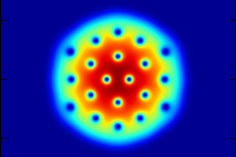
\includegraphics[width=0.5\textwidth]{density_L10_cut.png}
\end{center}
\column{0.5\textwidth}
\begin{center}
\onslide<2->
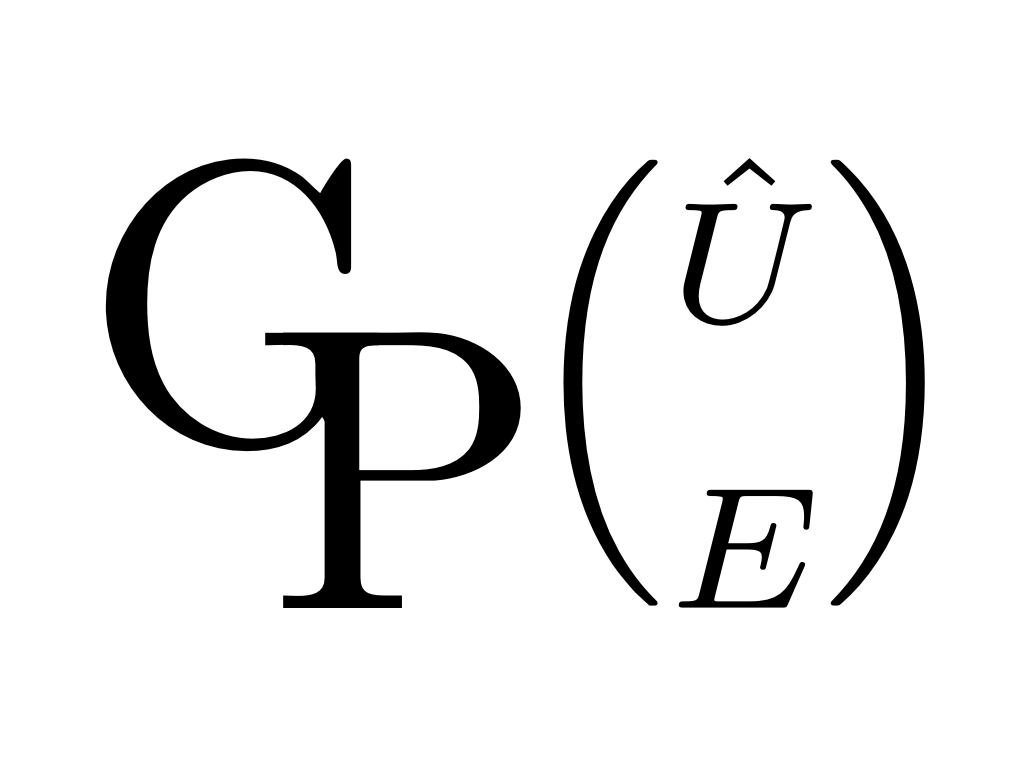
\includegraphics[width=0.5\textwidth]{GPUE.png}
\end{center}
\end{columns}

\end{frame}

\begin{frame}
\frametitle{What we will miss...}

\begin{columns}
\column{0.5\textwidth}
\center
\textbf{Physics: understanding superfluid vortices}

\vspace{0.5cm}
Quantum state engineering

{\scriptsize (\textit{NJP} 18 (3):035012, 2016)} \\
{\scriptsize \textbf{J Schloss}, A Benseny, J Gillet, J Swain, \\ T Busch} \\

\column{0.5\textwidth}
\center

\textbf{Computer Science: Spectral methods for GPUs}

\vspace{0.5cm}

Implementation details

{\scriptsize (Tests, formats, etc.)}
\vspace{0.7cm}

\end{columns}

\end{frame}

\begin{frame}
\frametitle{The Fourier Transform}

\begin{columns}
\onslide<1->
\column{0.5\textwidth}
Fourier Transform:
\begin{align*}
F(\xi) &= \int_{-\infty}^{\infty}f(t)e^{-2\pi i t \xi}dt\\
f(t) &= \int_{-\infty}^{\infty}F(\xi)e^{2\pi i t \xi}d\xi
\end{align*}

\onslide<3->
Discrete Fourier Transform:
\begin{align*}
X_k &= \sum_{n=0}^{N-1} x_ne^{2\pi i k n / N}\\
x_n &= \frac{1}{N}\sum_{k=0}^{N-1} X_ke^{-2\pi i k n / N}
\end{align*}

\onslide<4->
The FFT is a \textit{global} operation requiring iteration or recursion
\column{0.5\textwidth}
\onslide<2->
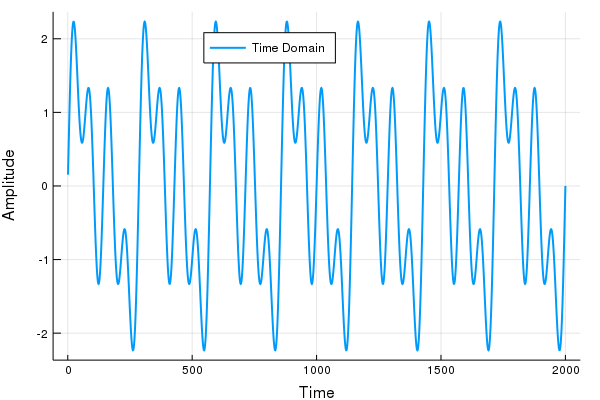
\includegraphics[width=\textwidth]{time_0066.png}
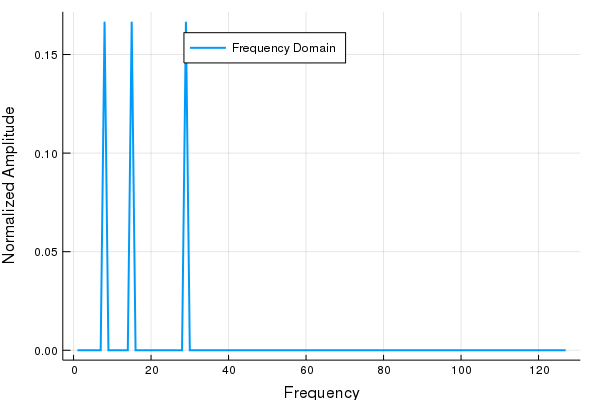
\includegraphics[width=\textwidth]{freq_0066.png}
\end{columns}
\end{frame}


\begin{frame}
\frametitle{Hamiltonian}
1D Schr\"odinger equation:
\begin{equation*}
i\hbar \frac{\partial \Psi(x, t)}{\partial t} = \left({\color{red}{\frac{ p^2}{2m}}} + {\color{blue}{\frac{1}{2}m\omega^2x^2}} \right)\Psi(x,t) \pause = \mathcal{H} \Psi(x,t)
\end{equation*}

Splits into:
\begin{columns}
\column{0.5\textwidth}
$$
\color{blue}{\mathcal{H}_v = \frac{1}{2}m\omega^2x^2}
$$
\column{0.5\textwidth}

\vspace{-0.8cm}
$$
\color{red}{\mathcal{ H}_p = \frac{p^2}{2m} = \frac{1}{2m}\left(i\hbar \frac{\partial}{\partial x}\right)^2}
$$
\end{columns}

\begin{center}
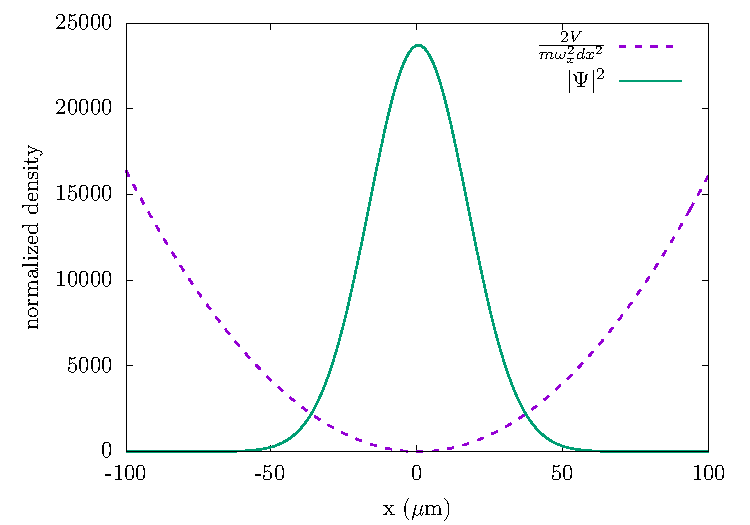
\includegraphics[width=0.5\textwidth]{../data/qs/SHO/SHO_2.pdf}
\end{center}
\end{frame}


\begin{frame}
\frametitle{Split-Step Fourier Method (SSFM)}

Differential Equations:

\begin{equation*}
\Psi(x,t + dt) = \left[e^{-\frac{i\mathcal{{H}}dt}{\hbar}}\right]\Psi(x,t) = \left[e^{-\frac{i({\color{blue}{\mathcal{{H}}_v}} + {\color{red}{\mathcal{{H}}_p}})dt}{\hbar}}\right]\Psi(x,t)
\end{equation*}

\pause
Baker-Campbell-Hausdorff:
\begin{equation*}
\Psi(x,t+dt) = \left[e^{-\frac{i{\color{blue}{\mathcal{{H}}_v}}dt}{\hbar}}e^{-\frac{i{\color{red}{\mathcal{{H}}_p}}dt}{\hbar}}e^{-\frac{[i{\color{blue}{\mathcal{{H}}_v}}, i{\color{red}{\mathcal{{H}}_p}}]dt^2}{2}}\right]\Psi(x,t)
\end{equation*}

Matrices:
\begin{columns}
\column{0.5\textwidth}
$$
\color{blue}{{U}_v = e^{-\frac{i\mathcal{{H}}_vdt}{\hbar}}}
$$
\column{0.5\textwidth}
$$
\color{red}{{U}_p = e^{-\frac{i\mathcal{{H}}_pdt}{\hbar}}}
$$
\end{columns}


\begin{equation*}
\Psi(x, t+dt) = \mathcal{F}^{-1}\left[{\color{red}{{U}_p(dt)}} \mathcal{F} \left[{\color{blue}{{U}_v(dt)}} \Psi(x,t) \right] \right] + \mathcal{O}(dt^2)
\end{equation*}

\end{frame}

\begin{frame}
\frametitle{Bose-Einstein condensation}
Bosons condense into a superfluid at slightly above 0 Kelvin

\begin{center}
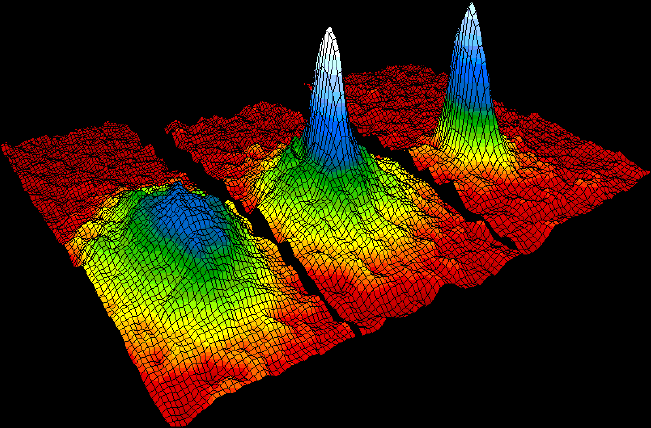
\includegraphics[width=0.5\textwidth]{Bose_Einstein_condensate.png}

\tiny{NIST/JILA/CU-Boulder}
\end{center}

\pause

Described by the mean field Gross--Pitaevskii equation:
\begin{equation*}
    i\hbar \frac{\partial}{\partial t}\Psi(x,t) = \left( - \frac{\hbar^2}{2m} \nabla^2 + \frac{1}{2}m\omega^2x^2 + {\color{red}{g |\Psi(x,t)|^2}}\right)\Psi(x,t)
\end{equation*}


\end{frame}

\begin{frame}
\frametitle{Superfluid rotation}
\center Rotation leads to many vortices along the axis of rotation
\vspace{0.25cm}

\begin{columns}
\column{0.4\textwidth}
Fluid
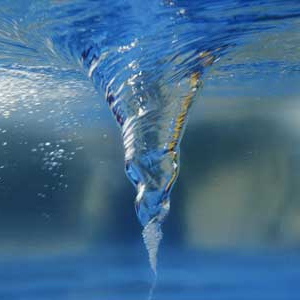
\includegraphics[width=\textwidth]{vortex.jpg}
\tiny{Credit: howstuffworks.com}
\pause
\column{0.40\textwidth}
Superfluid
\includegraphics[width=\textwidth]{vortexlattice.jpg}
\tiny{Credit: Peter Engels, JILA}
\end{columns}

\pause
\begin{equation*}
    i\hbar \frac{\partial}{\partial t}\Psi(x,t) = \left( - \frac{\hbar^2}{2m} \nabla^2 + V_0(x) + g |\Psi(x,t)|^2 {\color{red}{-\Omega L_z}} \right)\Psi(x,t)
\end{equation*}
$$
L_z = (xp_y - yp_x) = -i\hbar\left(x\frac{\partial}{\partial y} - y\frac{\partial}{\partial x} \right)
$$

\end{frame}

\begin{frame}
\center
\Huge{How do we create more complicated vortex structures?}
\end{frame}

\begin{frame}
\frametitle{Superfluid vortex phase}

\begin{center}
\includegraphics<1>[width=0.8\textwidth]{WIP_1.png}

\includegraphics<2>[width=0.8\textwidth]{WIP_2.png}

Each vortex has a $2\pi$ complex phase winding, $v \sim \nabla\phi$
\end{center}
\end{frame}

\begin{frame}
\frametitle{Phase imprinting}
\begin{center}
\includegraphics<1>[width=0.75\textwidth]{phase_1.png}

\includegraphics<2>[width=0.75\textwidth]{phase_2.png}

Phase masks can induce dynamical vortices
\end{center}

\end{frame}

\begin{frame}
\frametitle{Artificial magnetic fields}
\begin{center}
Magnetic fields cause rotation in \textit{charged} particles
\end{center}
\begin{columns}
\column{0.7\textwidth}
\begin{itemize}
\onslide<2->
\item The Hamiltonian of a particle with the Lorentz force law is:
$$
\mathcal{H} = \frac{(p-q\mathbf{A}(x))^2}{2m}, \qquad \mathbf{B} = \nabla\times\mathbf{A}
$$
\onslide<3->
\item Vortices follow the magnetic field lines
\onslide<4->
\item Modified GPE:
\begin{equation*}
\mathcal{ H} = \frac{(p-{\color{red}{m\mathbf{A}}} )^2}{2m} + V_0 + g|\Psi(x,t)|^2
\end{equation*}
\end{itemize}
\onslide<5->
\column{0.3\textwidth}
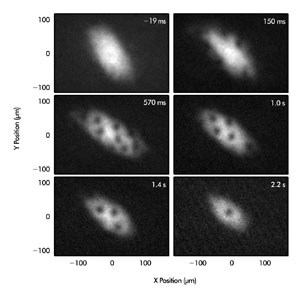
\includegraphics[width=\textwidth]{exp_synth.jpg}
\center{\tiny Ian Spielman, NIST}
\end{columns}
\end{frame}


\begin{frame}
\frametitle{Modifications to the GPE}
With gauge fields, the GPE becomes
\begin{equation*}
\mathcal{ H} = \frac{(p-{\color{red}{m\mathbf{A}}} )^2}{2m} + V_0 + g|\Psi(x,t)|^2
\end{equation*}

\onslide<2->
Which creates

\begin{columns}
\column{0.5\textwidth}
\onslide<2->
\begin{itemize}
\item A position-space component that couples with the trap
$$
\frac{m\mathbf{A}^2}{2}
$$

\onslide<3->
\item Components in position and momentum-space, that \textbf{require 1D FFT's}
$$
-\left(\frac{p\mathbf{A} + \mathbf{A}p}{2}\right)
$$
\end{itemize}
\onslide<2->
\column{0.55\textwidth}
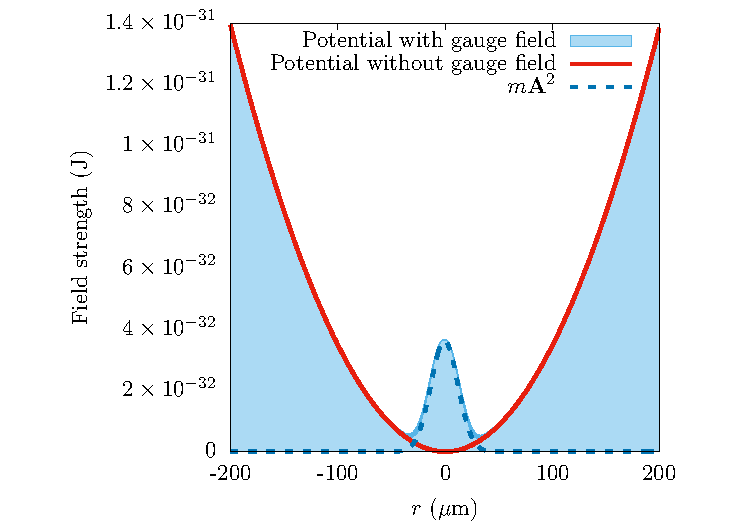
\includegraphics[width=1.1\textwidth]{../data/splitop/gauge/check.pdf}
\end{columns}

\end{frame}

\begin{frame}
\frametitle{Takeaways}
\begin{columns}
\hspace{0.25cm} \column{0.7\textwidth}
Physics
\begin{itemize}
\item Quantized vortices can be formed with rotation, phase imprinting, and artificial magnetic fields
\end{itemize}

Computer Science
\begin{itemize}
\item The SSFM requires a large number of FFT's
\item This system is a great for testing spectral methods
\end{itemize}
\hspace{-0.3cm} \column{0.3\textwidth}
 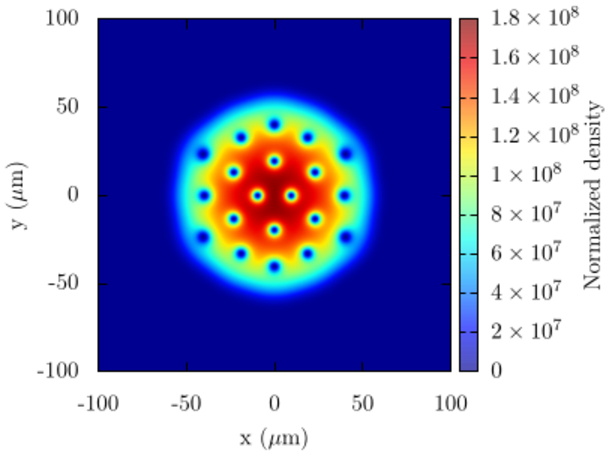
\includegraphics[width=1\textwidth]{../data/splitop/rot/density_L10.pdf}
\end{columns}

\end{frame}

\begin{frame}
\center \huge GPU computing and the GPUE codebase
\center{\scriptsize J Schloss, LJ O'Riordan \\
\textit{Journal of Open Source Software} 3 (32):1037, 2018}
\end{frame}

\begin{frame}
\frametitle{What is a GPU?}

\begin{columns}
\column{0.6\textwidth}
\begin{itemize}
\item Graphics processing units (GPUs) are massively parallel computing devices
\onslide<2->
\item GPUs are fast for parallel tasks
\onslide<3-> 
\item Summit uses GPUs
\end{itemize}
\onslide<1->
\center{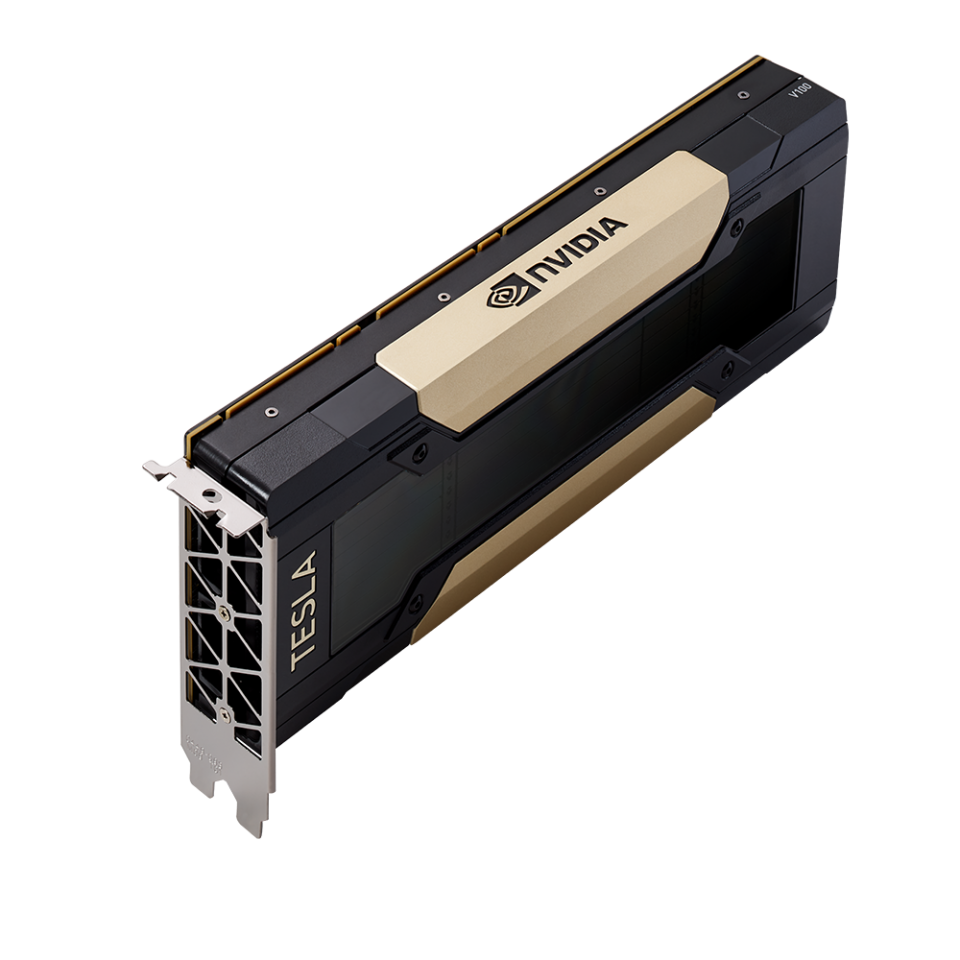
\includegraphics[width=0.7\textwidth]{v100.png}}

\column{0.4\textwidth}
\onslide<2->
\center{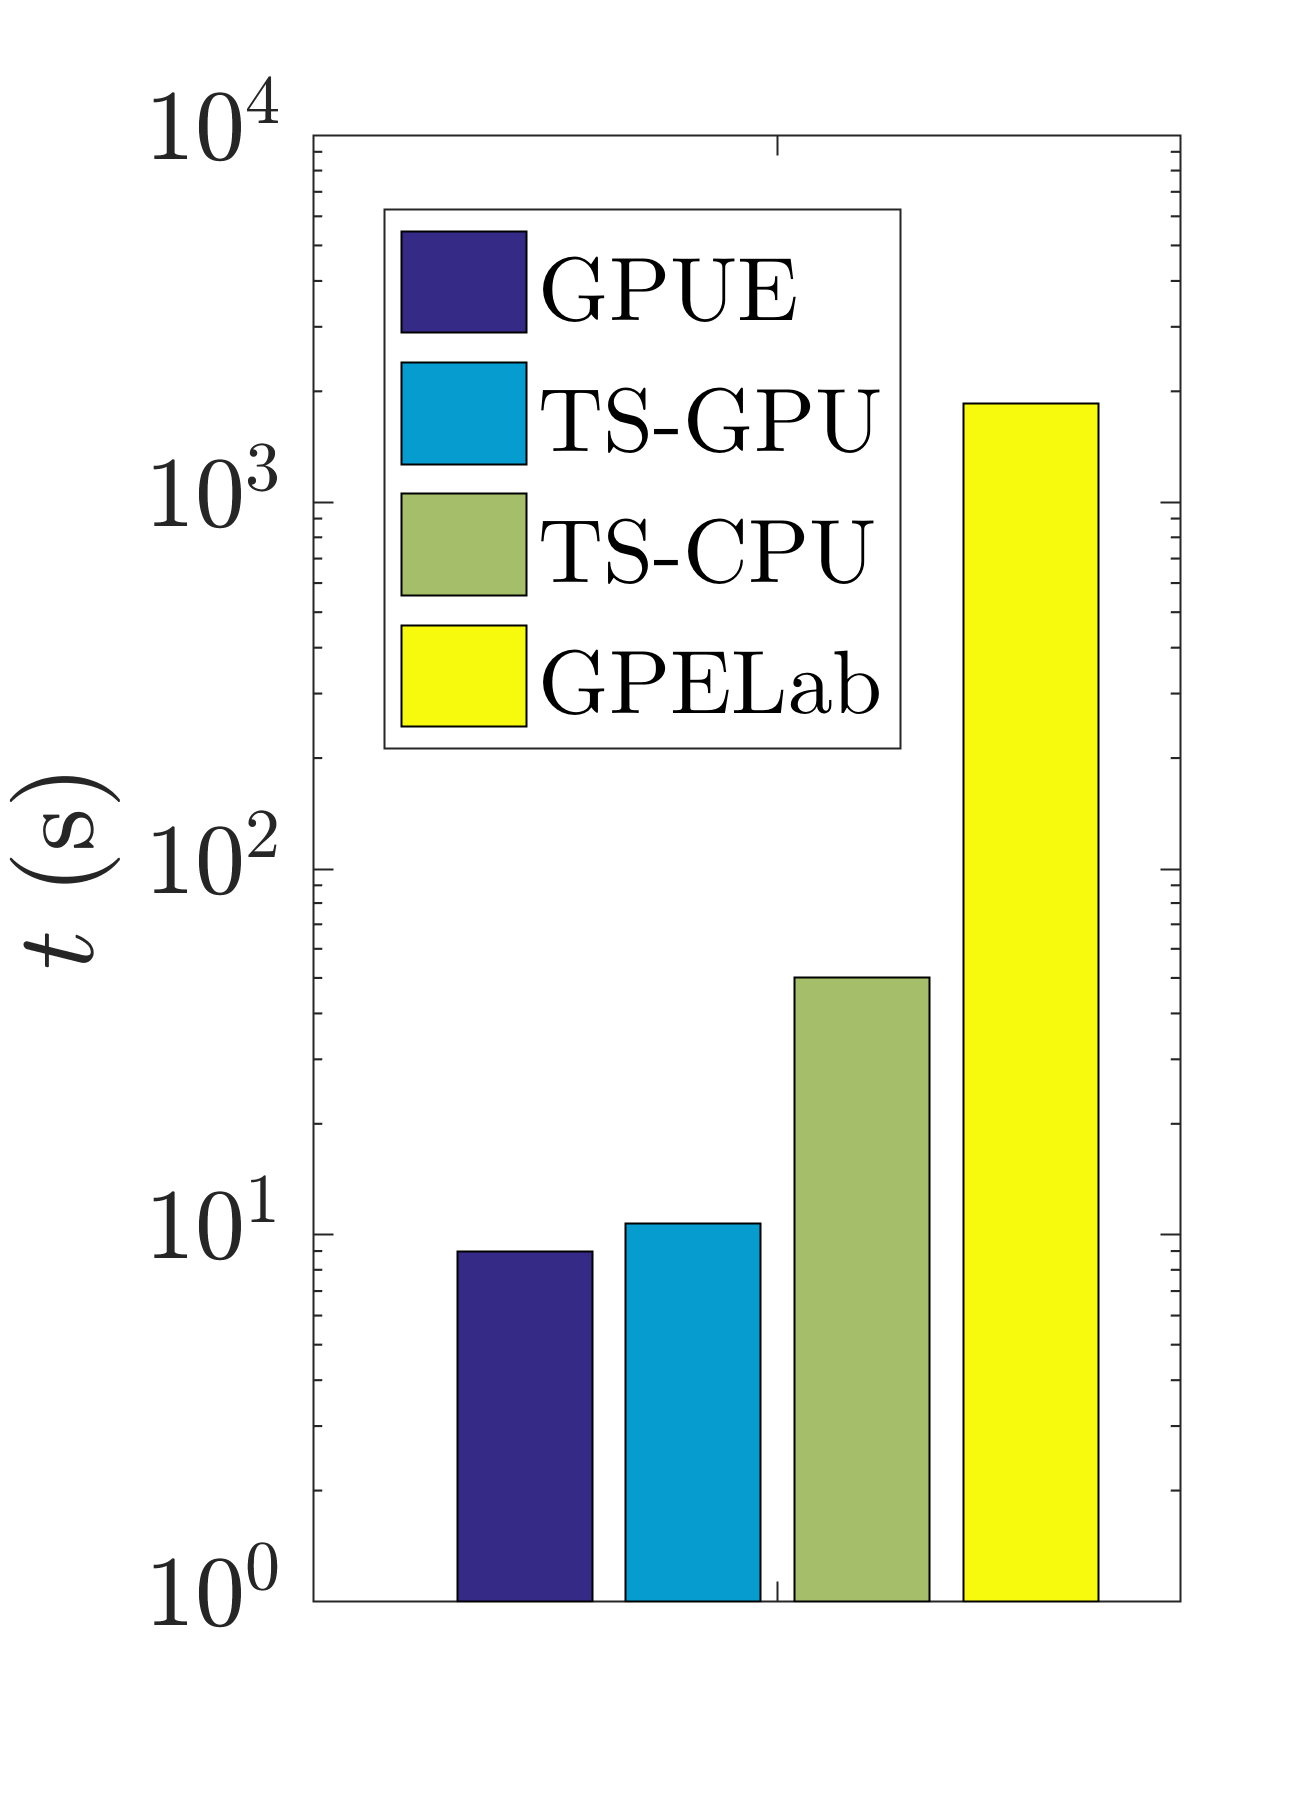
\includegraphics[width=\textwidth]{bench.png}}

\end{columns}

\onslide<2->

\end{frame}

\begin{frame}
\frametitle{GPU memory hierarchy}

\begin{columns}
\column{0.6\textwidth}
\begin{itemize}
\onslide<2->
\item Computing threads in blocks, blocks in grids
\onslide<3->
\item Memory coalescence
\onslide<4->
\item Data transfer is slow
\onslide<5->
\item Recursion and iteration is slow
\onslide<6->
\item Limited memory
\end{itemize}


\column{0.4\textwidth}
\onslide<2->
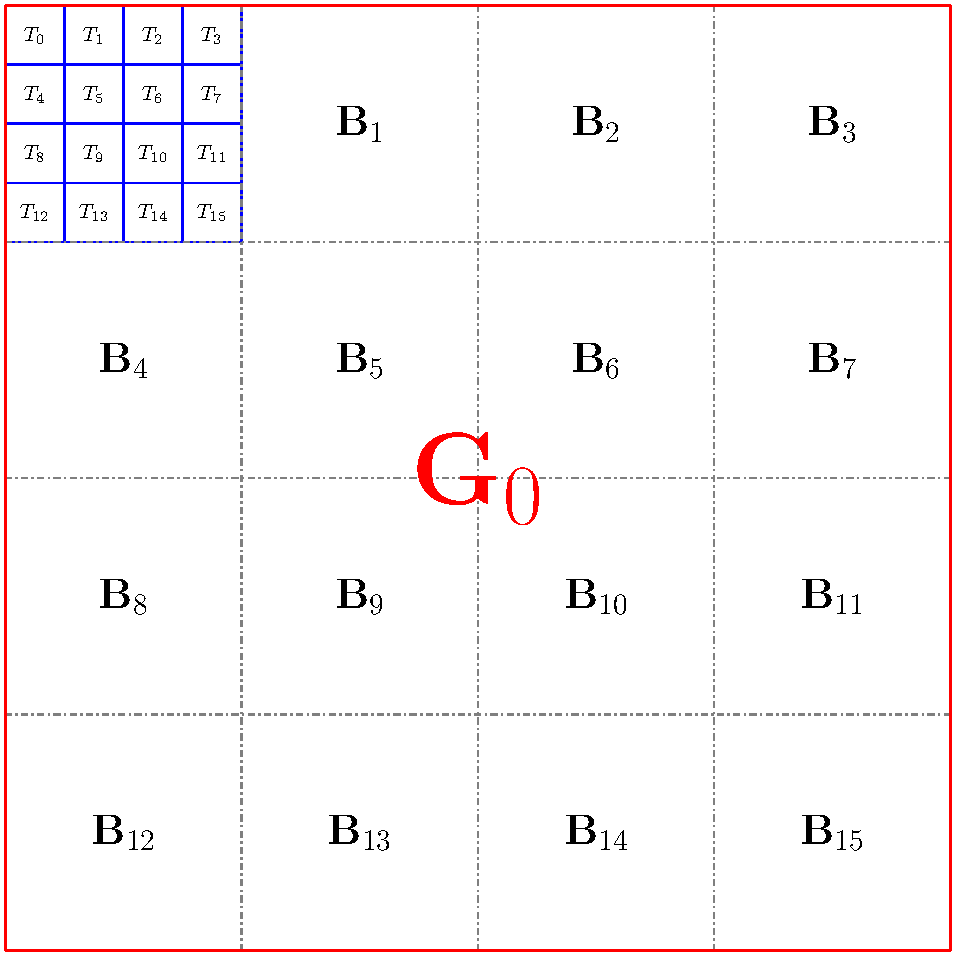
\includegraphics[width=\textwidth]{../data/gpu/gputhreads.pdf}
\end{columns}
\onslide<3->
\center{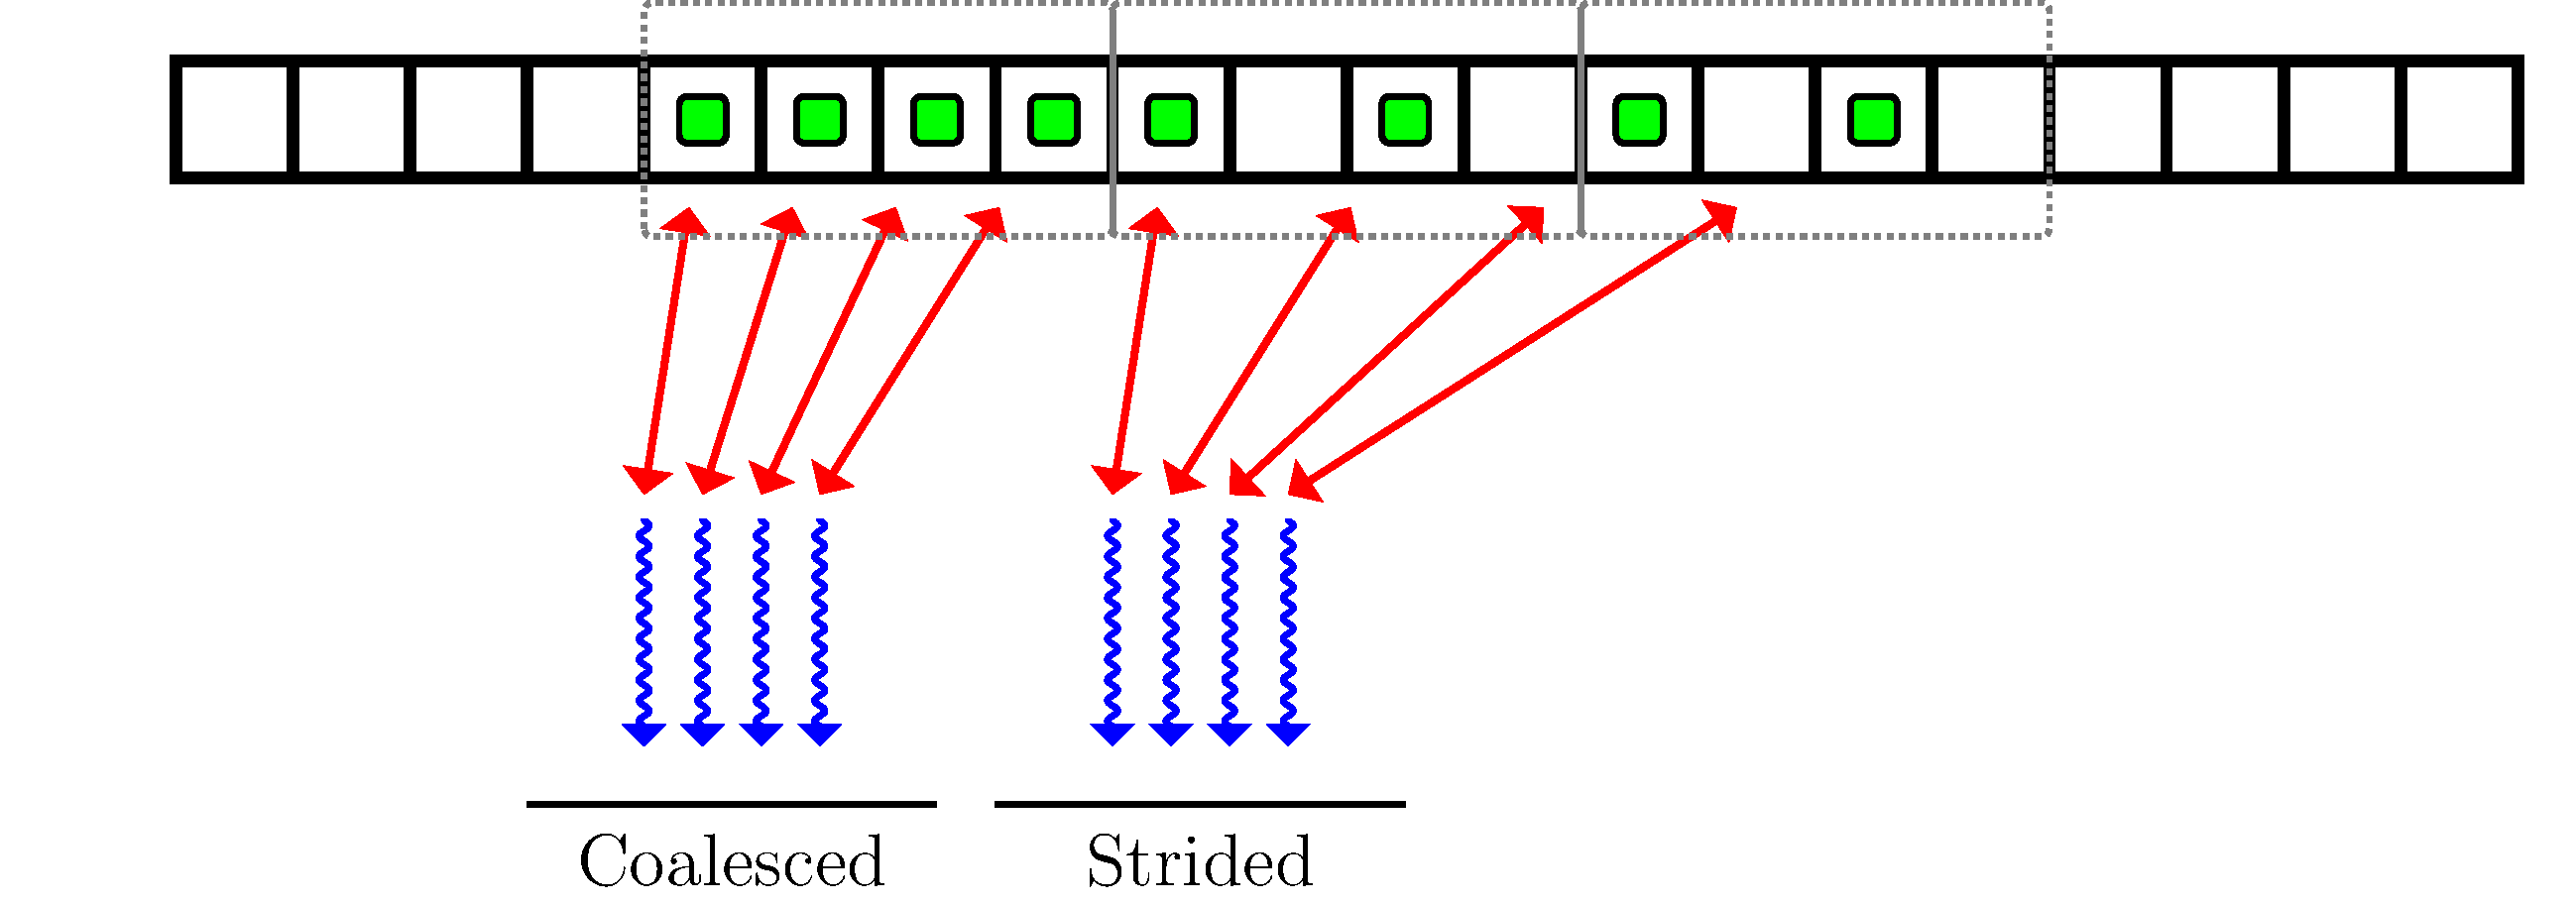
\includegraphics[width=0.8\textwidth]{../data/gpu/coalesce/check.pdf}}
\end{frame}

\begin{frame}
\frametitle{FFT notes}
\begin{columns}
\column{0.4\textwidth}
\begin{itemize}
\item Global operations
\item 1D FFT's are not supported by CuFFT
\pause
\item Transposes are necessary
\end{itemize}
\center 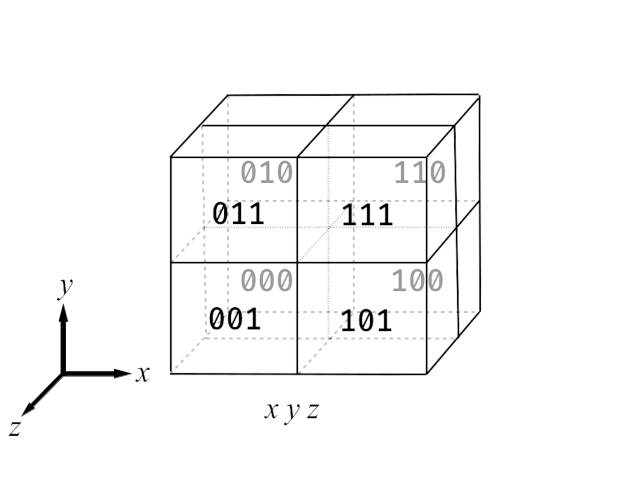
\includegraphics[width=\textwidth]{../data/gpu/fft/fft_fig.png}

\column{0.7\textwidth}
\center 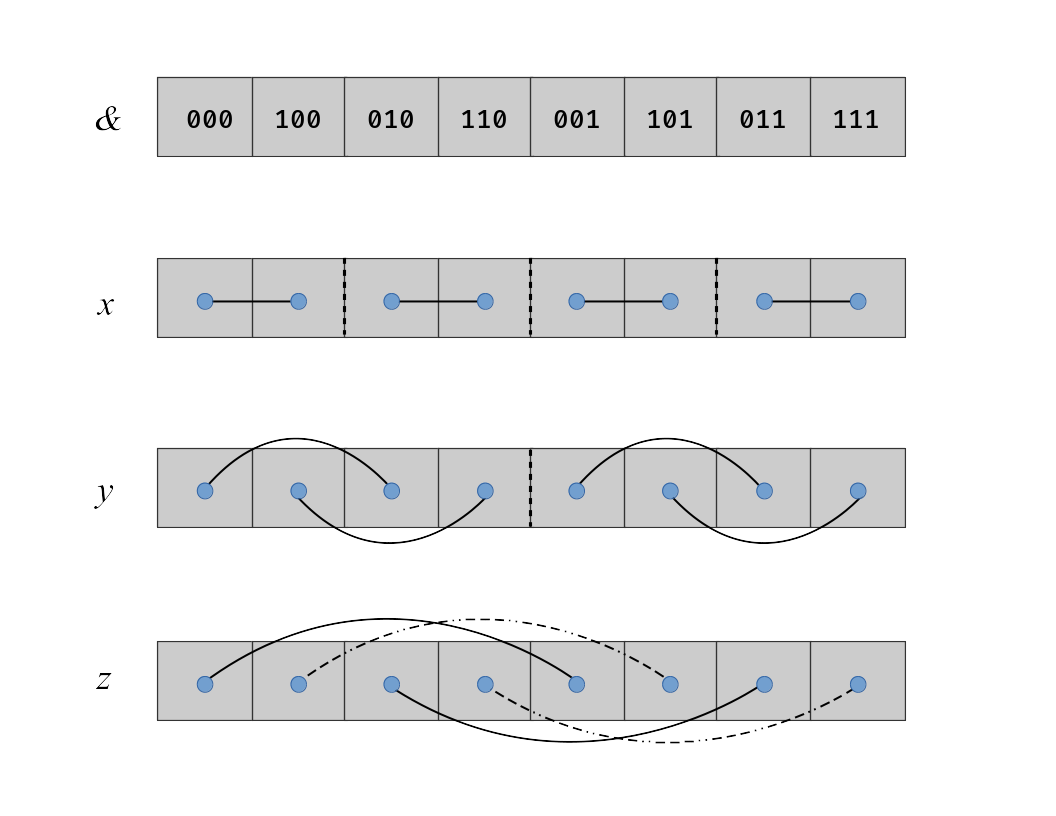
\includegraphics[width=\textwidth]{../data/gpu/fft/fft_fig2.png}
\end{columns}

\end{frame}

\begin{frame}
\center{\Huge Transposes are actually hard}

... We are working on it.

\end{frame}


\begin{frame}
\frametitle{Two important features}
\center{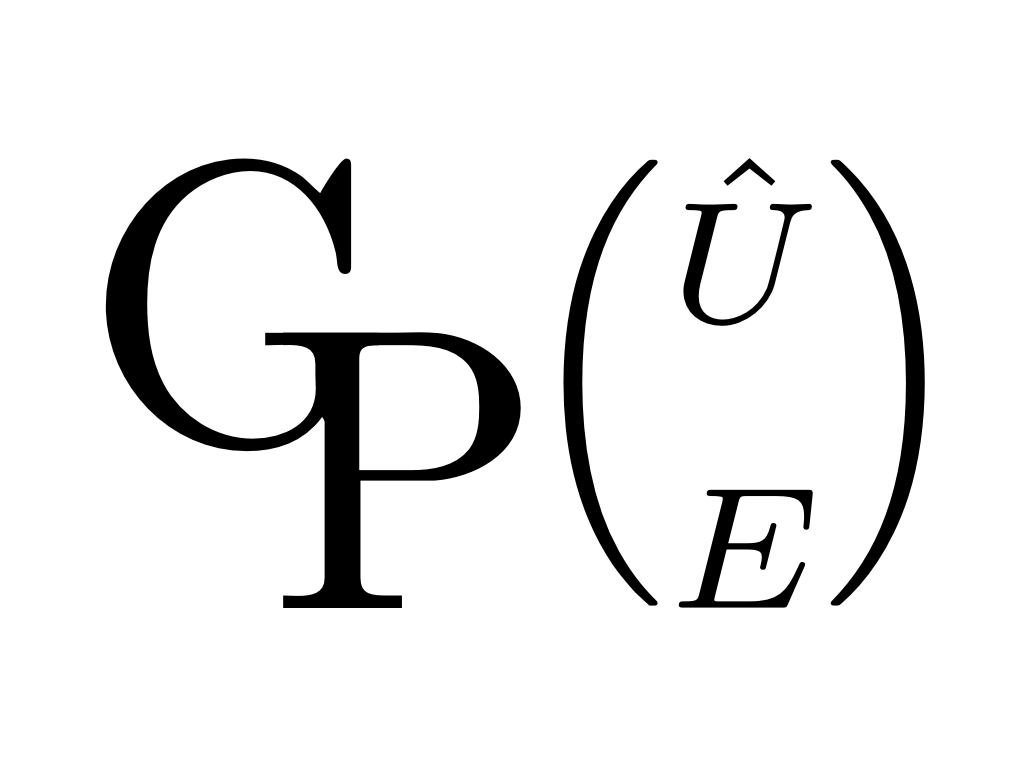
\includegraphics[width=0.5\textwidth]{GPUE.png}}

\begin{itemize}
\item Novel features useful for understanding examples
\item No discussion of implementation details
\end{itemize}
\end{frame}


\begin{frame}
\frametitle{Expression trees}
Notes:
\begin{itemize}
\item CUDA code is hard to write
\item Users want time-dependent fields for state engineering
\item GPUs have limited memory
\end{itemize}

\pause
\center 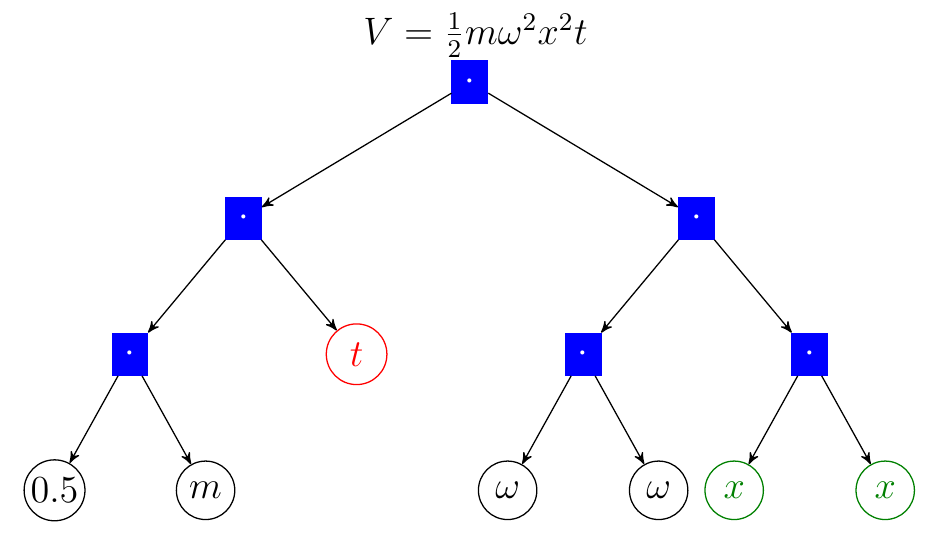
\includegraphics[width=0.6\textwidth]{expr_tree.png}
\end{frame}

\begin{frame}
\frametitle{Vortex tracking and highlighting}
\begin{columns}
\column{0.5\textwidth}
\begin{itemize}
\item Phase plaquettes in 2D
\onslide<2->
\item Vortex highlighting in 3D
\end{itemize}
\onslide<2->
\center 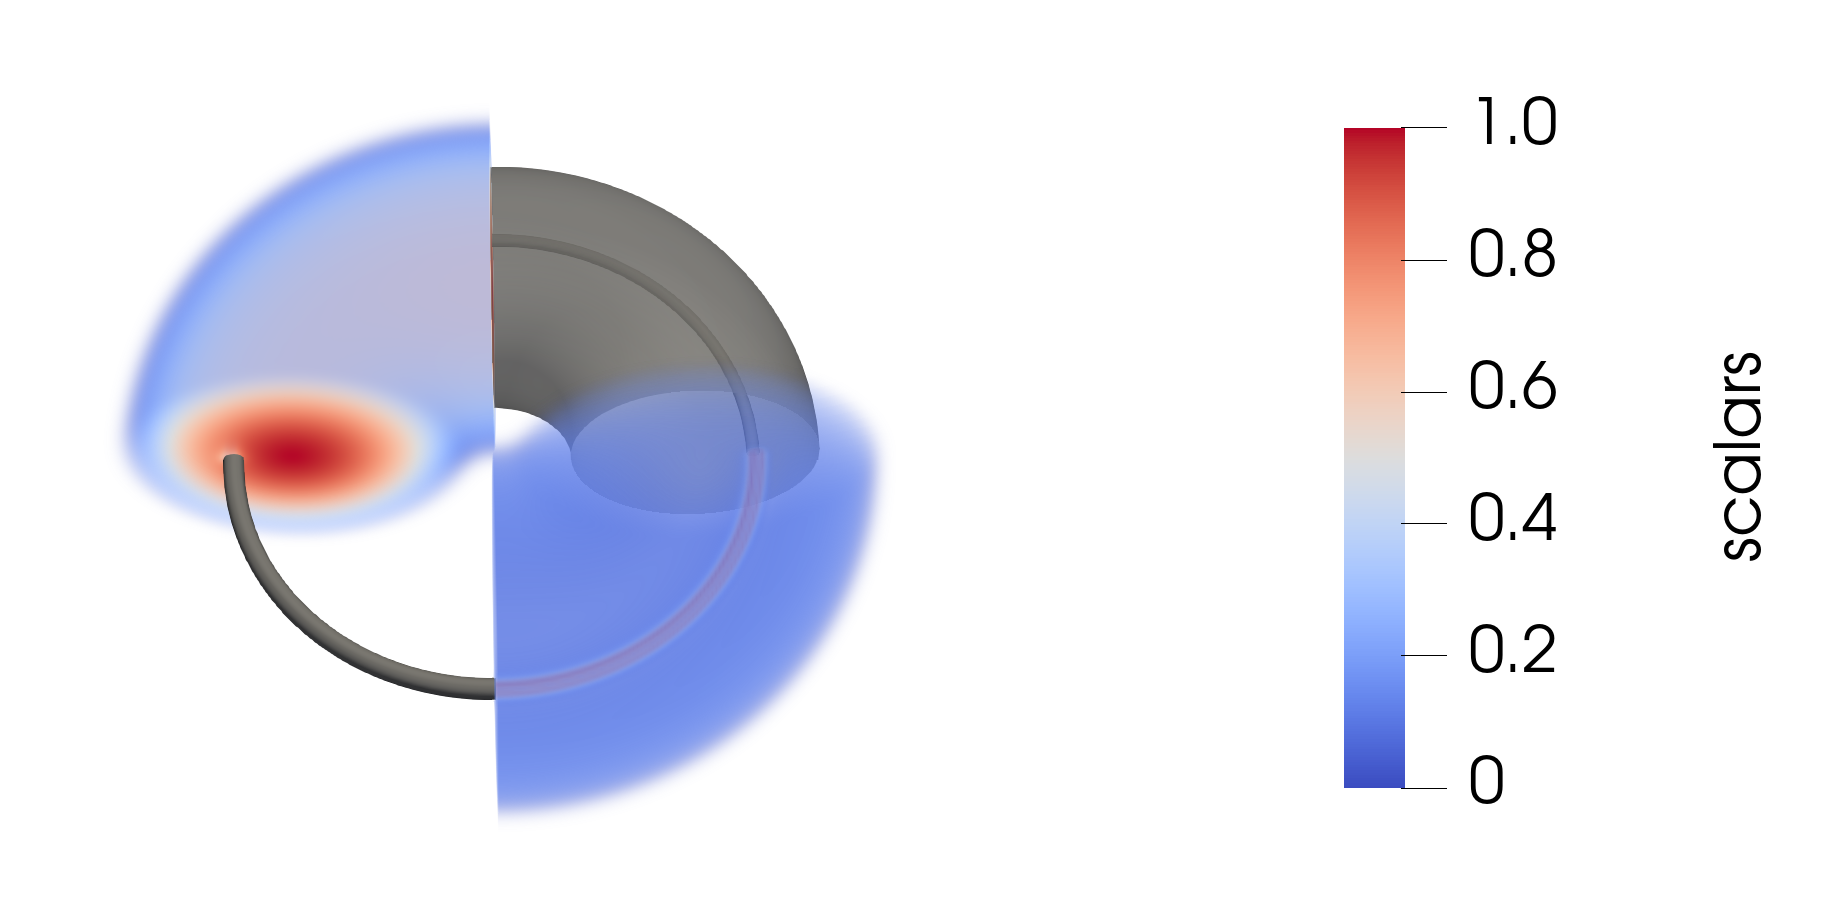
\includegraphics[width=1.2\textwidth]{../data/gpu/vortex_highlighting/all.png}
\column{0.5\textwidth}

\onslide<1->
\center 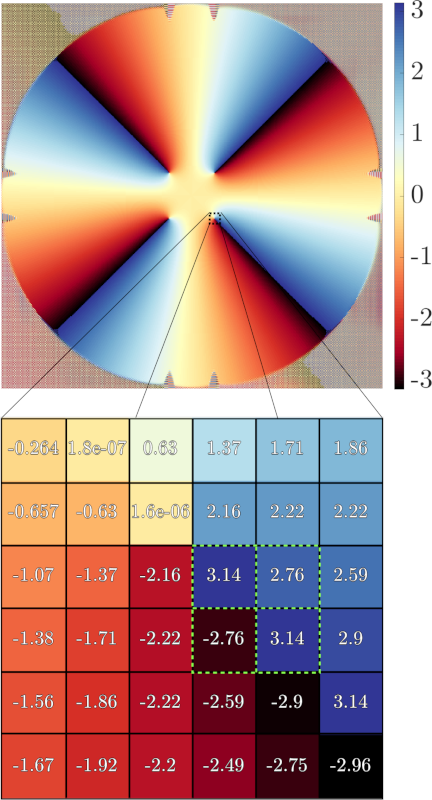
\includegraphics[width = 0.8\textwidth]{../data/gpu/vortex_tracking/phi_grid.png}

\end{columns}
\end{frame}

\begin{frame}
\frametitle{Takeaways}

Physics
\begin{itemize}
\item GPUE is fast, can do dynamic simulations, and vortex detection
\item Multi-component simulations and HDF5 have also been implemented
\end{itemize}

Computer Science
\begin{itemize}
\item The distributed transpose is hard
\item Expression trees save a lot of GPU memory when usable
\end{itemize}
\end{frame}

\begin{frame}
\center \huge Chaotic vortex dynamics in 2D BEC simulations
\center{\scriptsize T Zhang, \textbf{J Schloss}, A Thomasen, LJ O'Riordan, T Busch, A White \\
\textit{Physical Review Fluids} 4 (5):054701}
\end{frame}

\begin{frame}
\frametitle{3 vortex, 1 anti-vortex}

\includegraphics<1>[width=\textwidth]{histogram_1}

\includegraphics<2->[width=\textwidth]{histogram_2}

\onslide<3->
\center{\Huge Can we induce chaos?}

\end{frame}

\begin{frame}
\frametitle{Dynamics}

\end{frame}

\begin{frame}
\frametitle{Divergence in trajectories}
\begin{columns}

\column{0.6\textwidth}
Divergence in trajectory when Lyapunov exp ($\lambda$) becomes positive
$$
\delta \mathbf{P(t)} = (\delta x(t), \delta y(t), \delta v_x(t), \delta v_y(t))
$$
$$
|\delta\mathbf{P}(t)| \approx e^{\lambda t} |\delta \mathbf{P}_0|
$$
$$
\lambda = \lim_{t\to\infty}\frac{1}{t}\text{ln}\frac{||\delta\textbf{P}(t)||}{||\delta\textbf{P}(0)||}
$$

\column{0.4\textwidth}
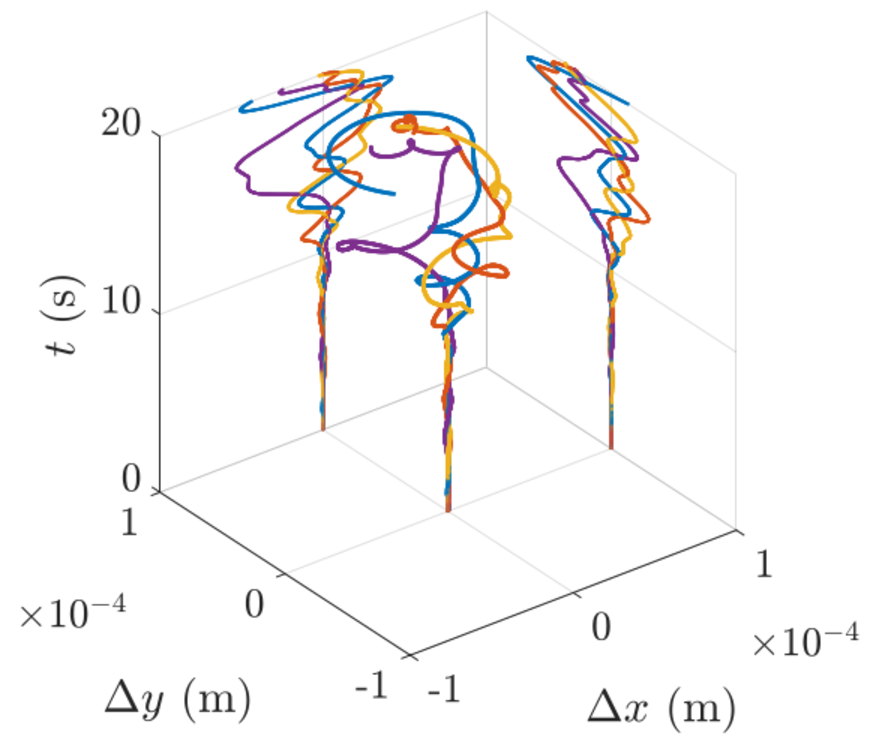
\includegraphics[width=\textwidth]{../data/2d/evolution/evolution}

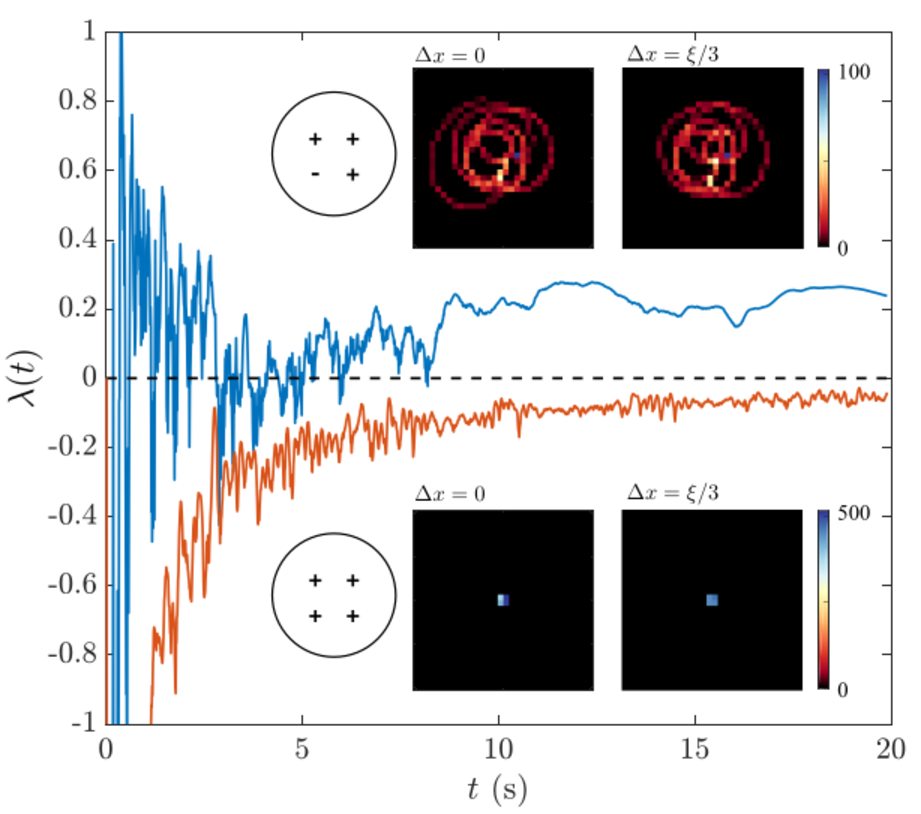
\includegraphics[width=\textwidth]{../data/2d/lyap/lyap}
\end{columns}
\end{frame}

\begin{frame}
\frametitle{Takeaway}
Physics
\begin{itemize}
\item \textit{Controlled} creation of chaotic dynamics
\item Chaotic dynamics of few-vortex systems is accelerated by collisional events
\end{itemize}
Computer Science
\begin{itemize}
\item 50 TB of data
\item Reliant on post-processing metrics (Lyapunov exp, Vortex tracking)
\item 1 hour per run (on K80's), infeasible with other software
\end{itemize}
\end{frame}

\begin{frame}
\center \huge 3D vortex ring generation in toroidal BEC systems
\center{\scriptsize J Schloss, P Barnett, R Sachdeva, T Busch \\
arXiv:1910.02364}
\end{frame}

\begin{frame}
\frametitle{Artificial magnetic fields}
\begin{center}
Magnetic fields cause rotation in \textit{charged} particles
\end{center}
\begin{columns}
\column{0.7\textwidth}
\begin{itemize}
\onslide<2->
\item If a two-level atom moves slowly in a tuned light field, \textit{Berry's connection} is
$$
\mathbf{A} = i\hbar\braket{\psi_l | \nabla\psi_l}
$$
\item The magnetic field is
$$
\mathbf{B} = \nabla \times \mathbf{A}
$$
\onslide<3->
\item Vortices follow the magnetic field lines
\end{itemize}
\onslide<2->
\column{0.3\textwidth}
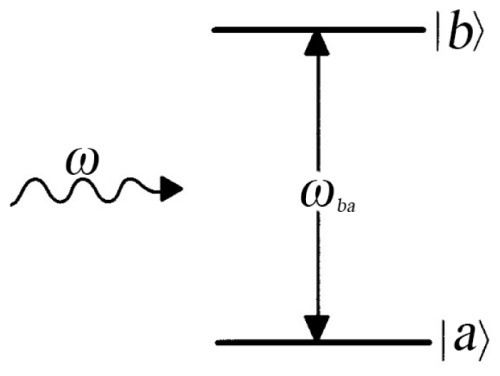
\includegraphics[width=\textwidth]{2level.jpg}
\end{columns}
\end{frame}


\begin{frame}
\frametitle{The system}

\begin{columns}

\onslide<2->
\column{0.7\textwidth}
\begin{itemize}
\item BEC toroidally trapped around nanofiber
\item Nanofiber generates $\mathbf{A}$
\item Vortices follow $\mathbf{B} = \nabla \times \mathbf{A}$
\end{itemize}

\column{0.3\textwidth}
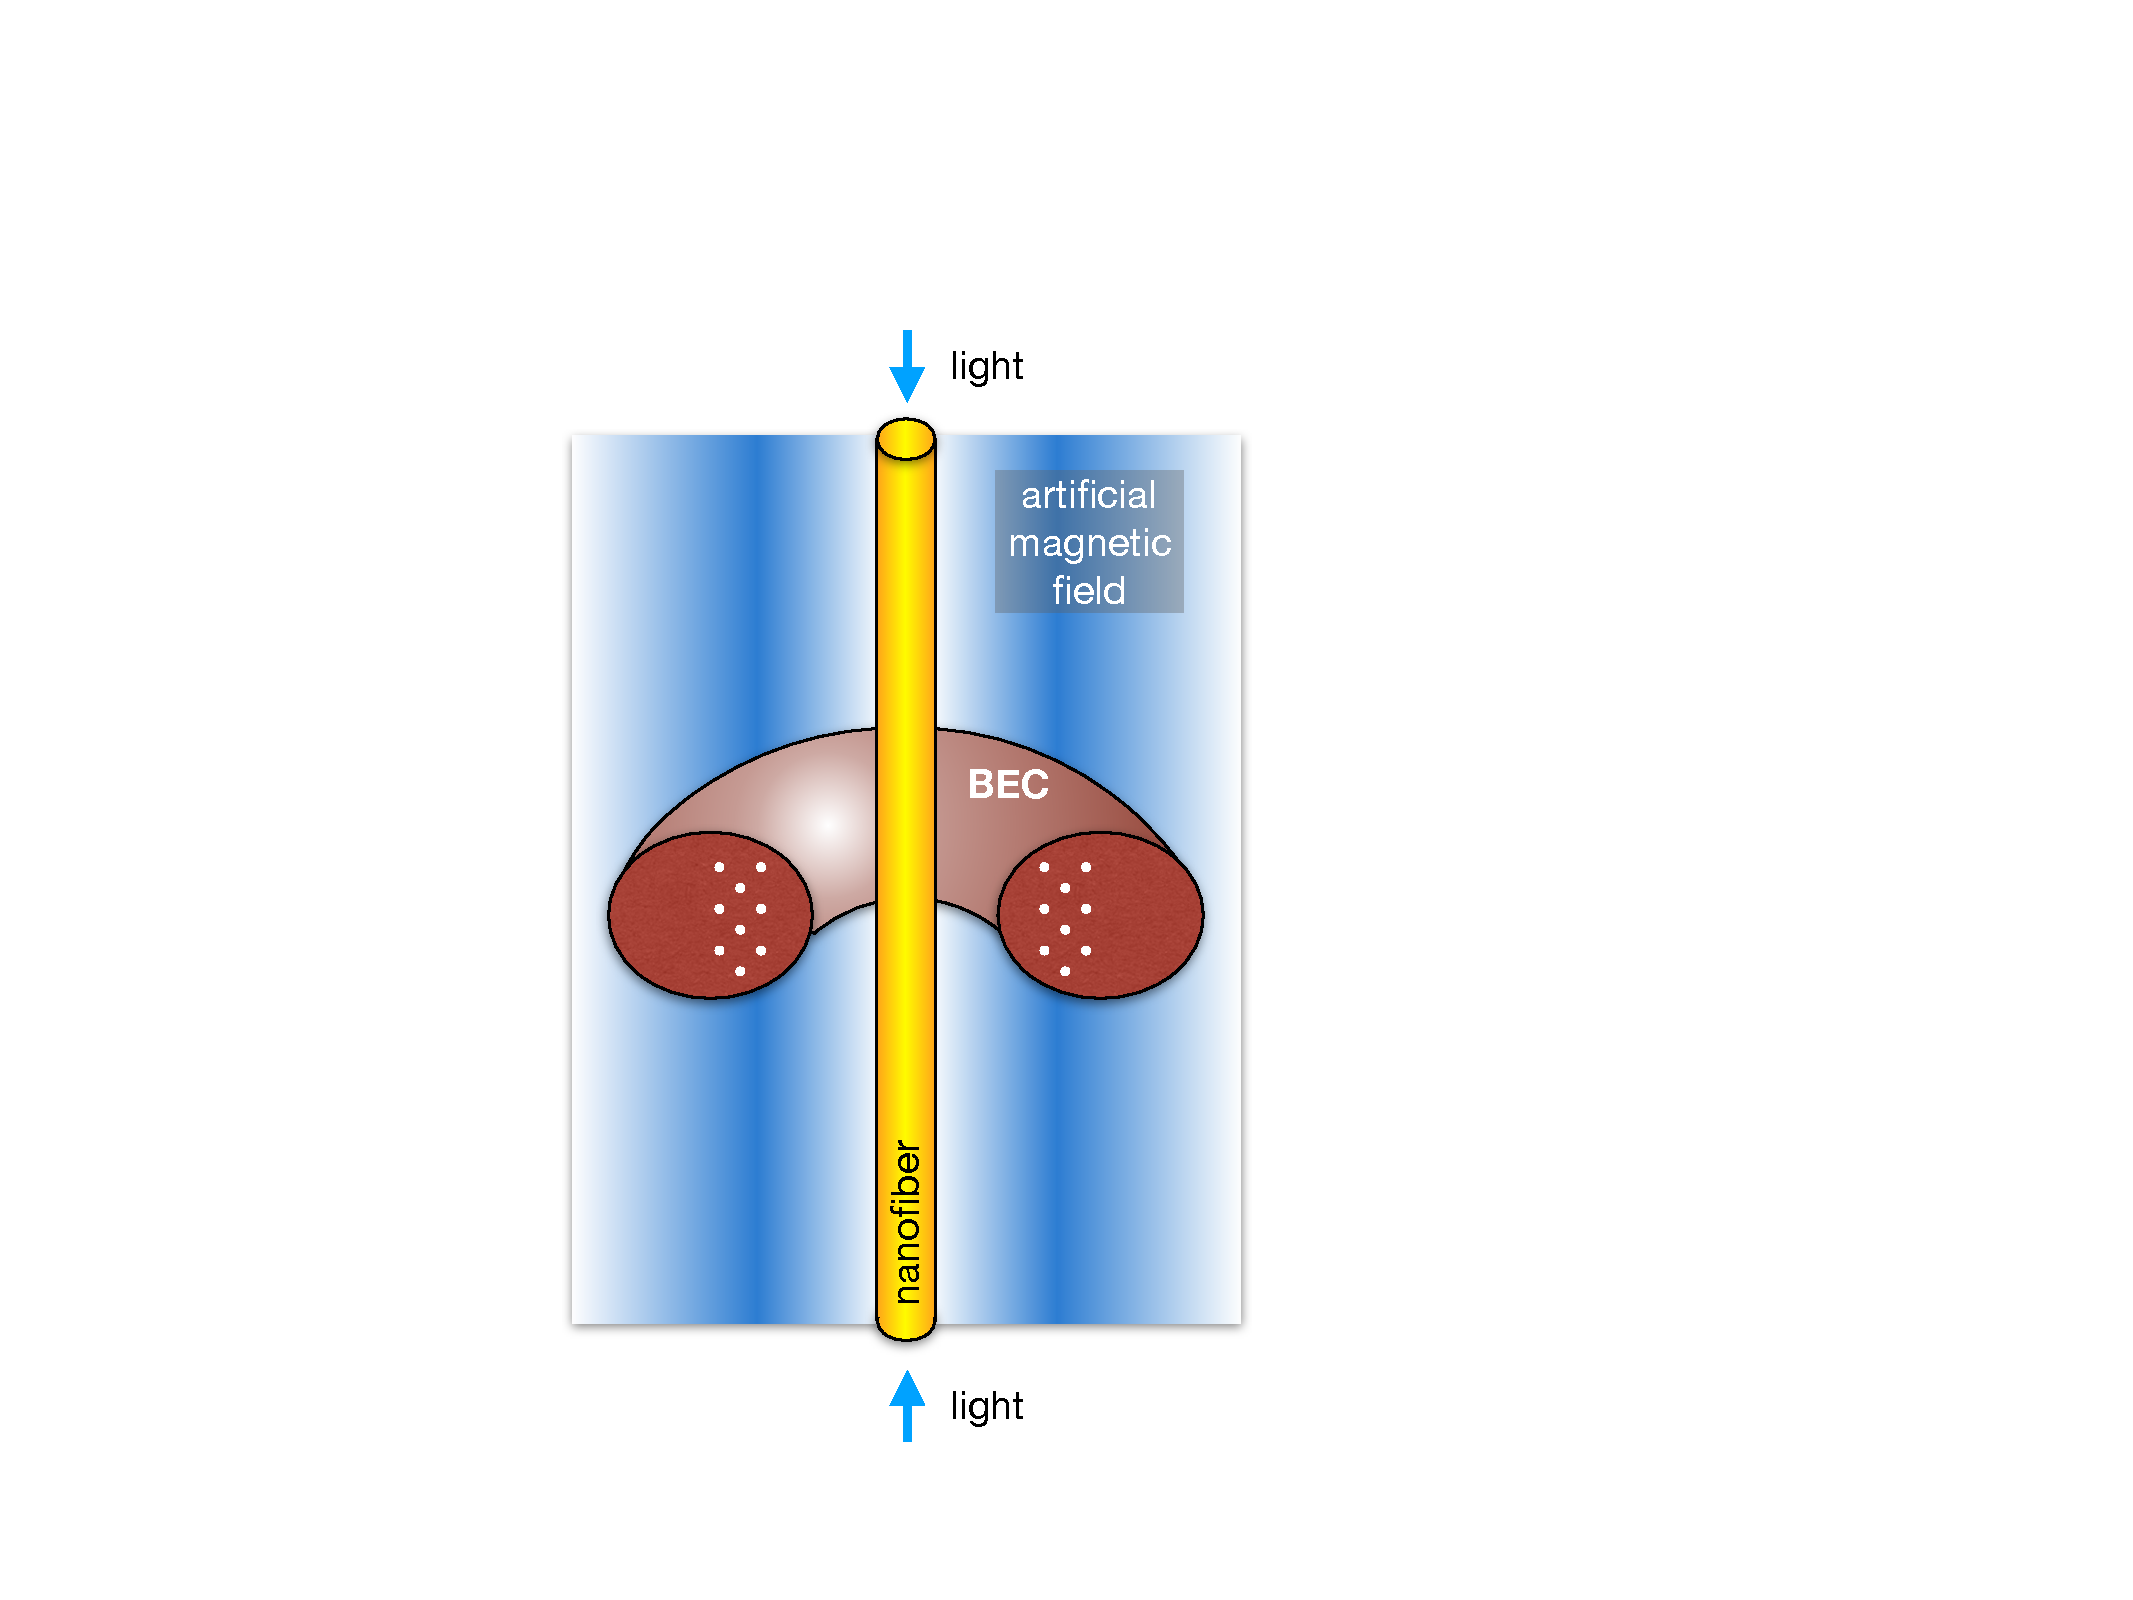
\includegraphics[width=\textwidth]{../data/3d/Schematic_TB}
\end{columns}

\onslide<1->
\center 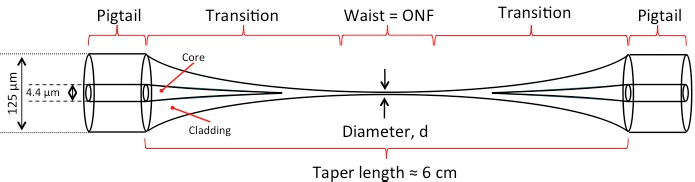
\includegraphics[width=0.8\textwidth]{nanofiber.png}

\tiny MJ Morrissey, K Deasy, M Frawley, R Kumar, E Prel, L Russell, VG Truong, and S Nic Chormaic \textit{Sensors} 13(8):10449-81, 2013

\end{frame}

\begin{frame}
\frametitle{Optical nanofiber}
\center 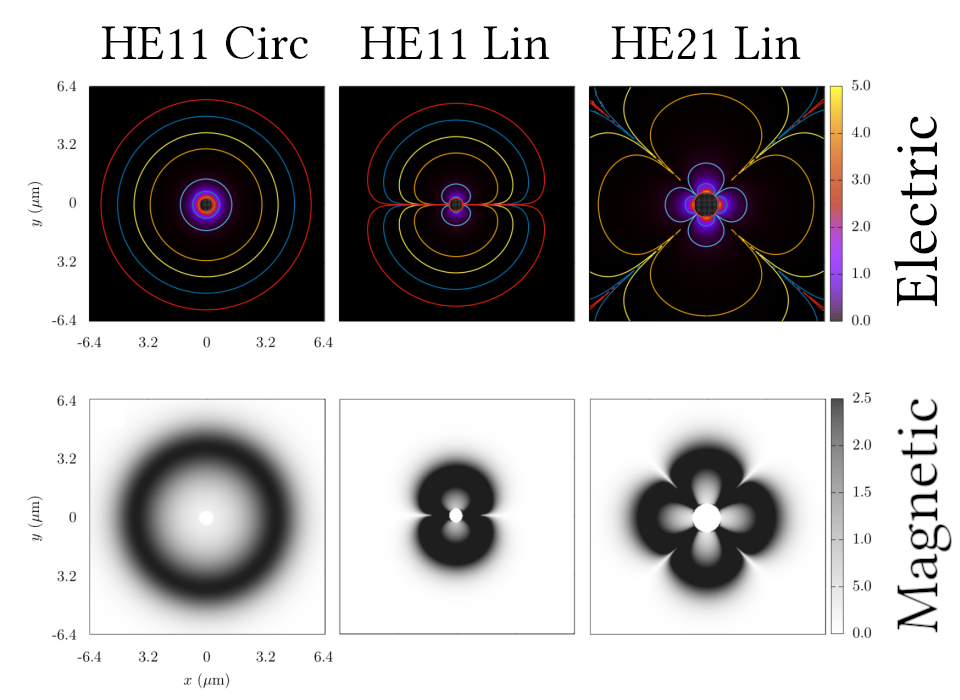
\includegraphics[width=0.8\textwidth]{all_fields.png}


\end{frame}

\begin{frame}
\frametitle{Vortex structures}
\begin{center}
\includegraphics<1>[width=\textwidth]{vortex_transition_1.png}

\includegraphics<2->[width=\textwidth]{vortex_transition_2.png}
\end{center}
\begin{columns}
\column{0.5\textwidth}
\begin{itemize}
\onslide<2->
\item Transition with linear polarization
\onslide<3->
\item Vortex structures align with $\mathbf{B}$
\end{itemize}
\column{0.5\textwidth}
\onslide<3->
\center 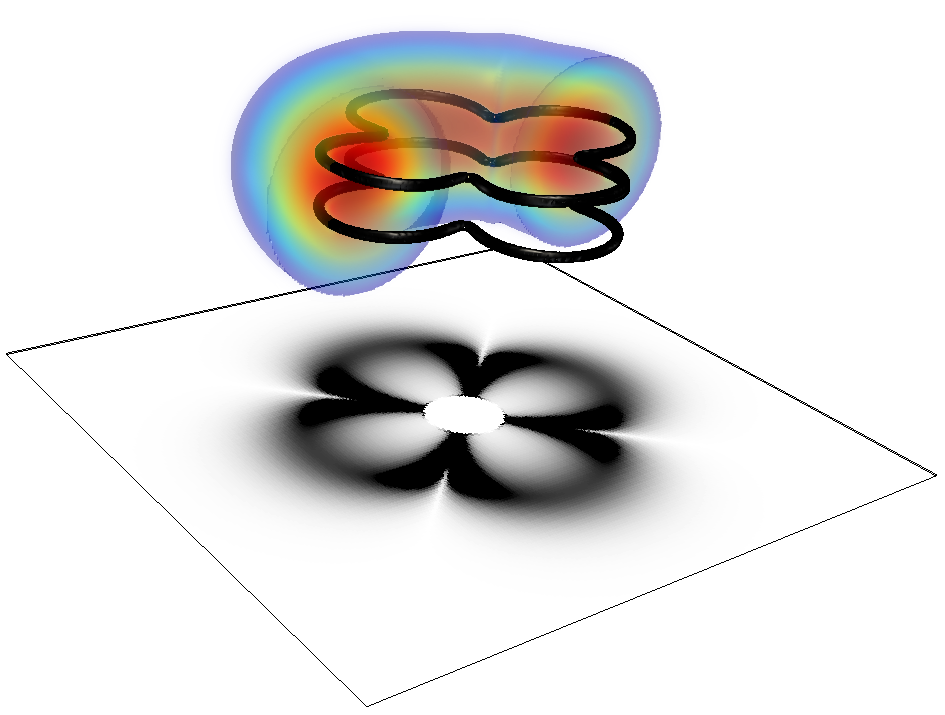
\includegraphics[width=\linewidth]{../data/3d/HE21_3d.png}
\end{columns}
\end{frame}

\begin{frame}
\frametitle{Vortex ring lattices}

\begin{columns}
\column{0.5\textwidth}
A vortex ring lattice can be generated with high $\mathbf{B}$
\column{0.5\textwidth}
\onslide<1->
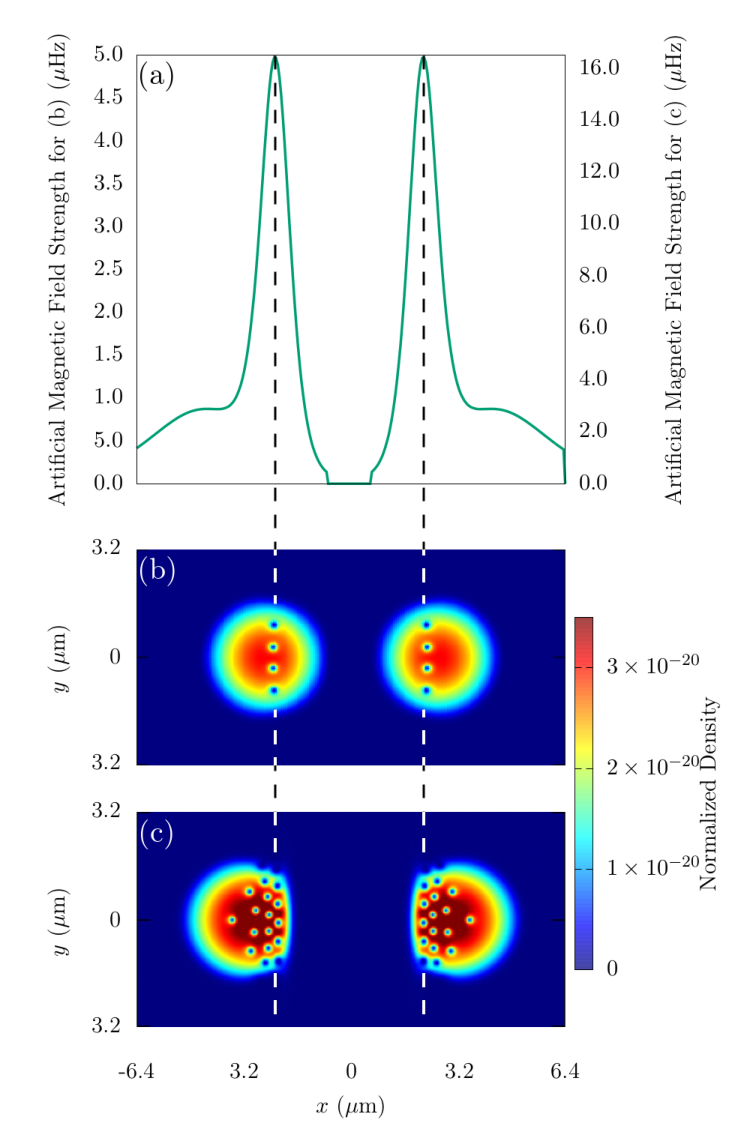
\includegraphics[width=\linewidth]{../data/3d/vortex_line_all.pdf}
\end{columns}
\end{frame}

\begin{frame}
\frametitle{Scissors modes}
\begin{itemize}
\item Vortex detection in 3D is difficult
\item Scissors modes provide different oscillations with vortices
\onslide<2->
\item First time shown for elliptic-toroidal trap
\end{itemize}
\begin{center}
\onslide<1->
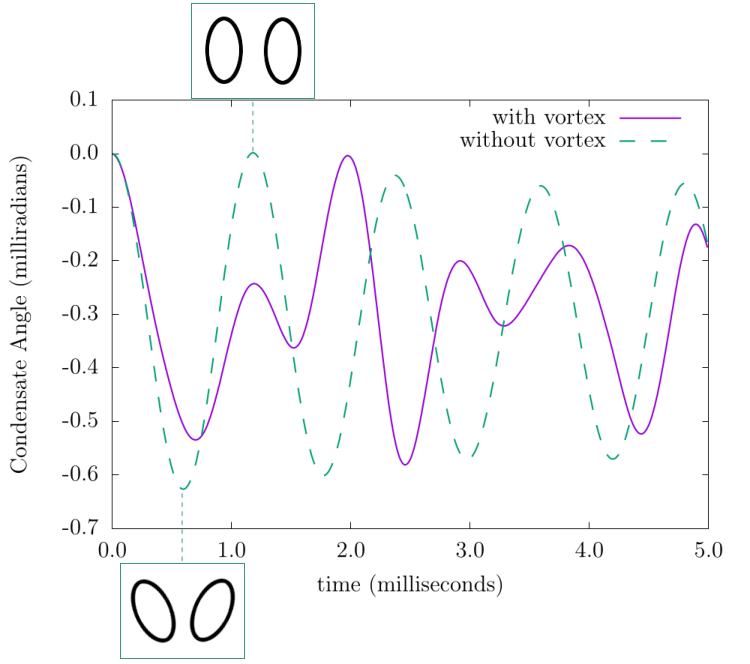
\includegraphics[width=0.6\textwidth]{../data/3d/scissors_plot.pdf}
\end{center}
\end{frame}

\begin{frame}
\frametitle{Takeaway}
Physics
\begin{itemize}
\item We can generate, control, and detect vortex structures in a BEC around a nanofiber
\item Dynamic simulations are underway!
\end{itemize}
Computer Science
\begin{itemize}
\item Dynamic simulations require a large amount of fileIO
\item Scaling to a larger grid requires multiple GPU's
\end{itemize}
\end{frame}


\begin{frame}
\center \huge Overall conclusions
\end{frame}

\begin{frame}
\frametitle{Overall conclusions}

\begin{columns}
\column{0.8\textwidth}
GPU computing is fast
\column{0.2\textwidth}
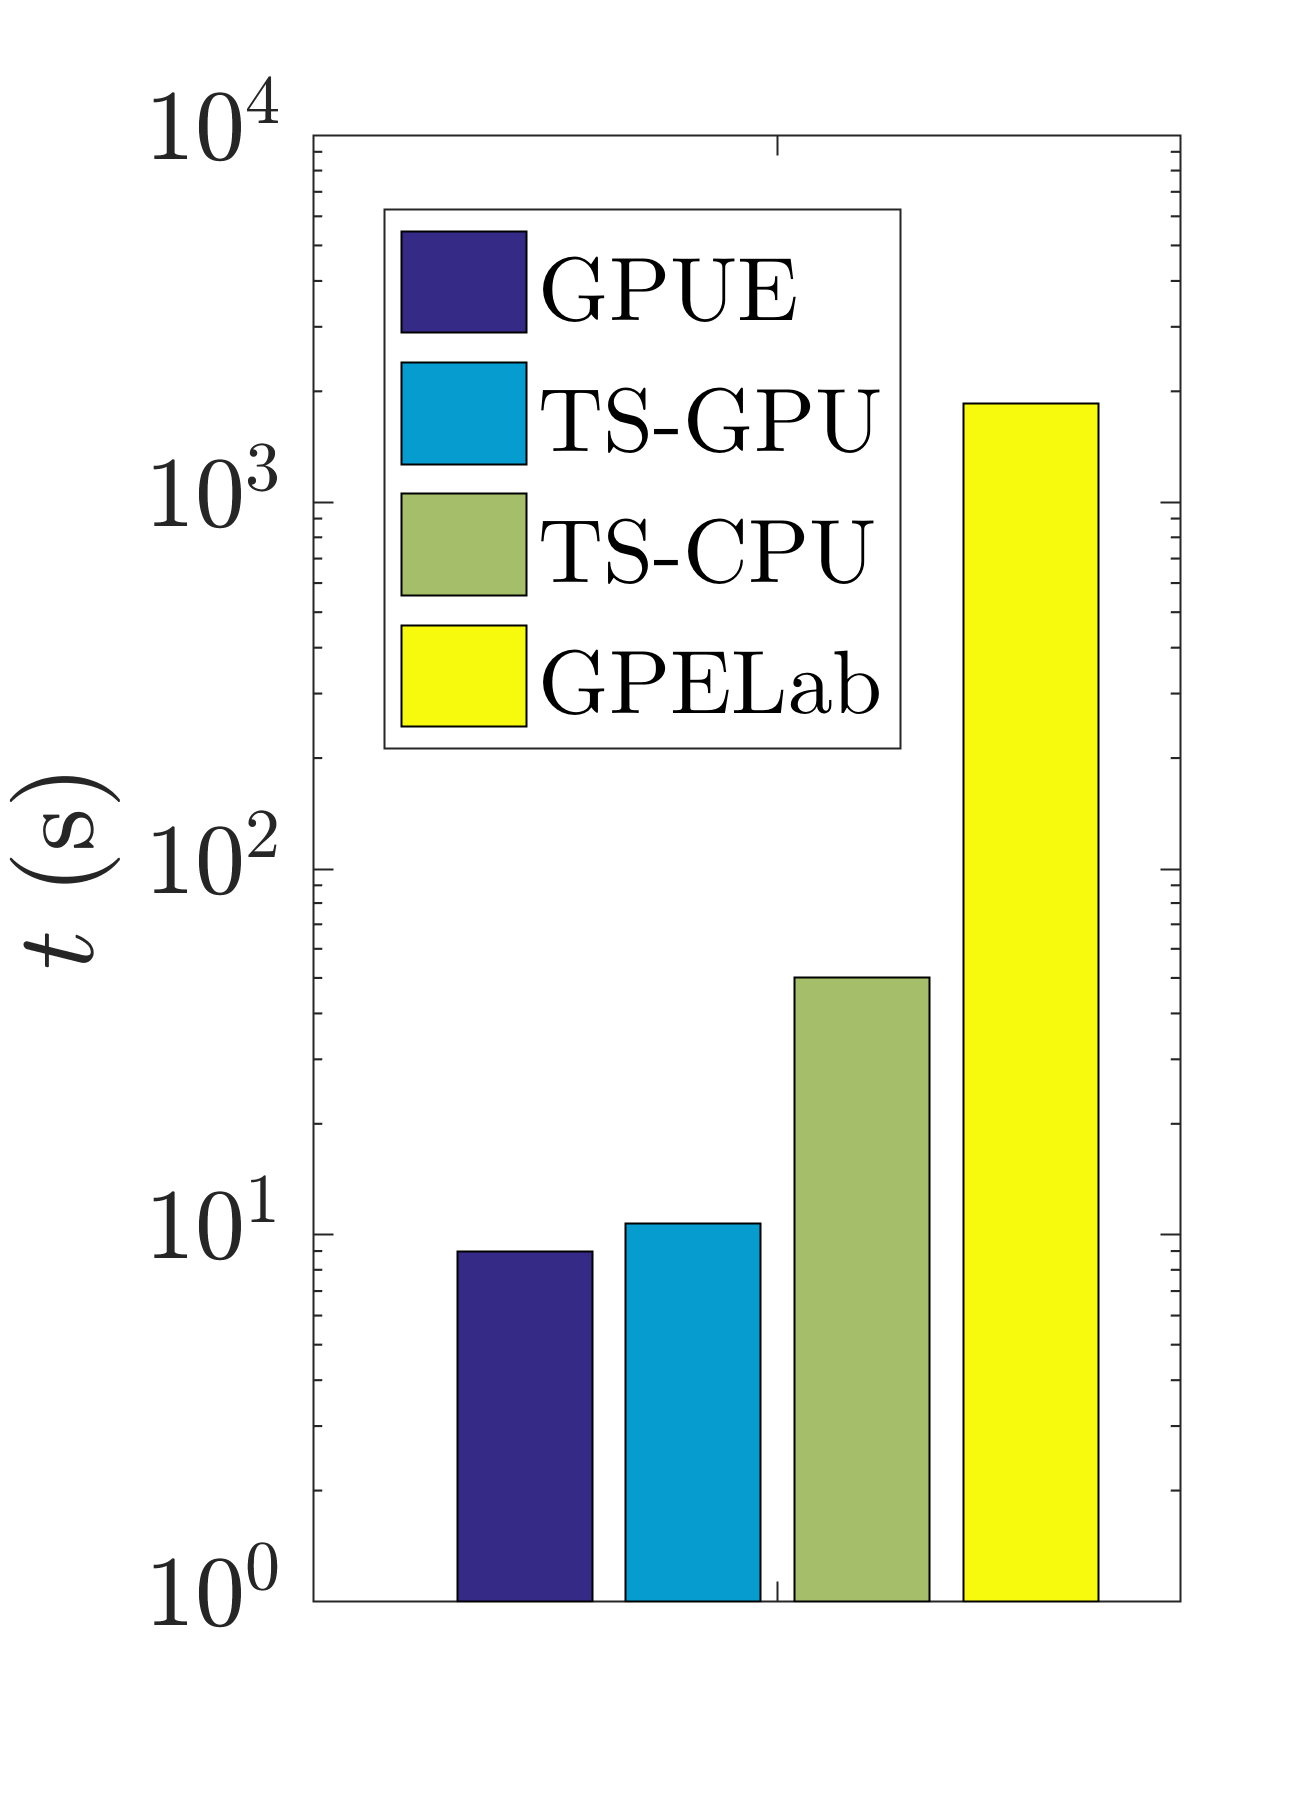
\includegraphics[width=\textwidth]{bench.png}
\end{columns}

\begin{columns}
\column{0.3\textwidth}
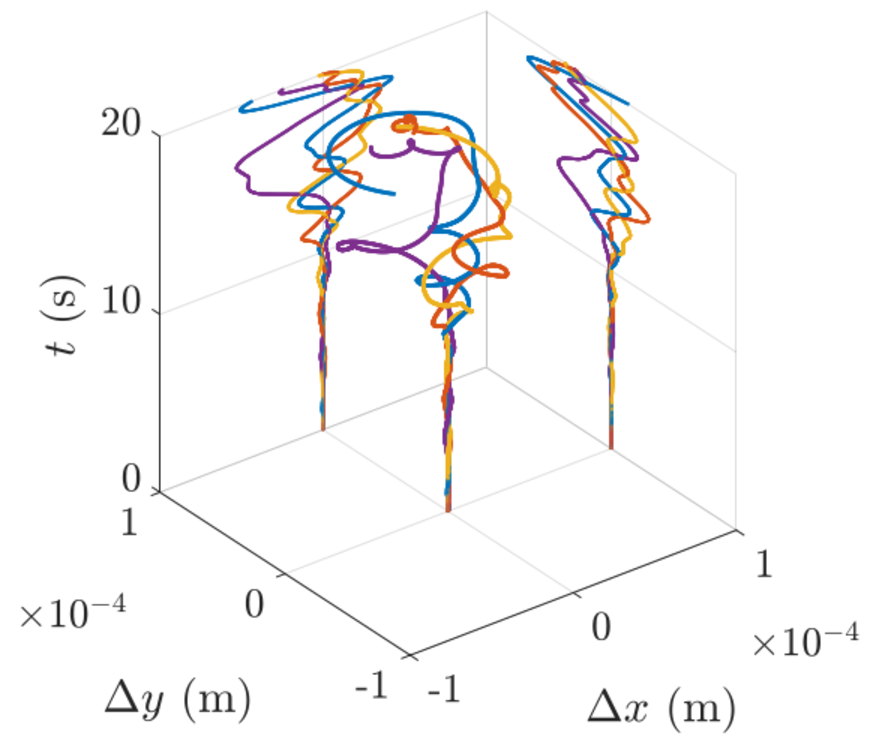
\includegraphics[width=\textwidth]{../data/2d/evolution/evolution}
\column{0.7\textwidth}
We can control chaos
\end{columns}

\begin{columns}
\column{0.7\textwidth}
We can control vortex structures
\column{0.3\textwidth}
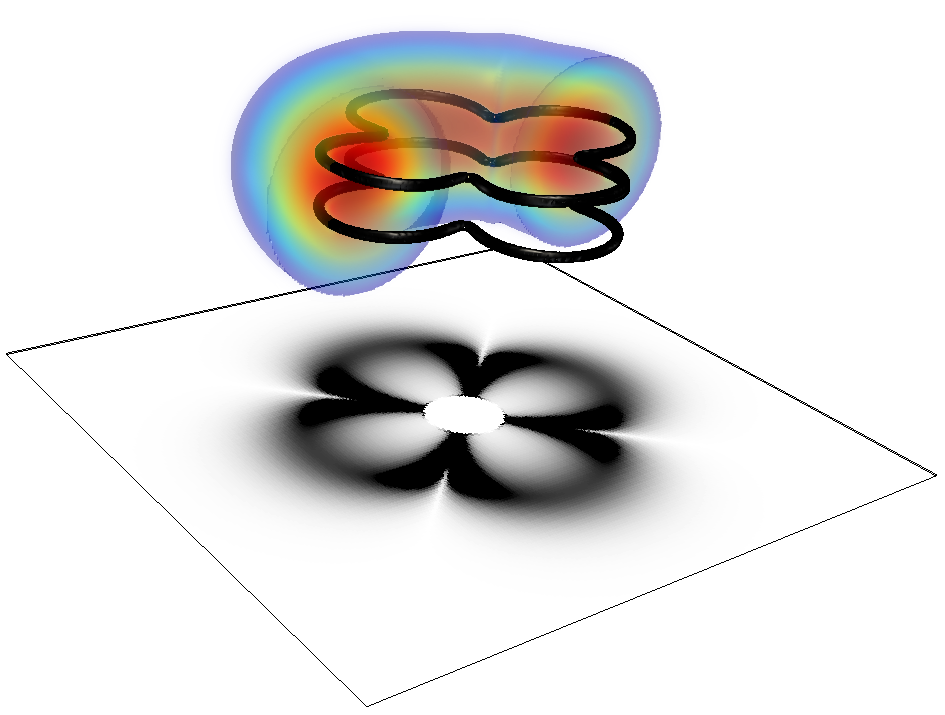
\includegraphics[width=\textwidth]{../data/3d/HE21_3d}
\end{columns}

\end{frame}

\begin{frame}
\frametitle{Future directions}
\begin{itemize}
\item Distributed Transpose
\item GPUE.jl
\item General-purpose Hamiltonian solver
\item Full vortex tracking
\item Octree-based gridding for SSFM
\end{itemize}
\end{frame}

\begin{frame}
\frametitle{People}
\begin{columns}
\column{0.7\textwidth}
\begin{columns}
\column{0.03\textwidth}
\column{0.15\textwidth}
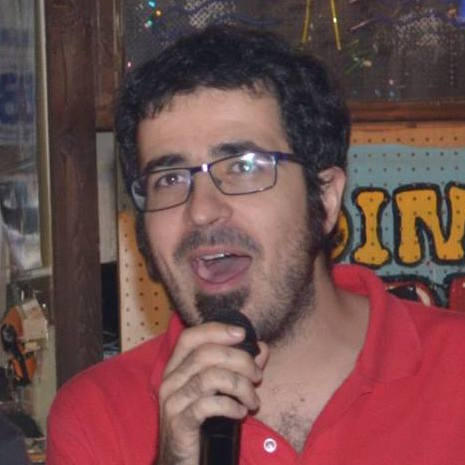
\includegraphics[width=\textwidth]{ABC.jpg}
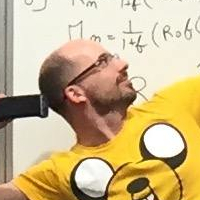
\includegraphics[width=\textwidth]{Jeremie.jpg}
\column{0.15\textwidth}
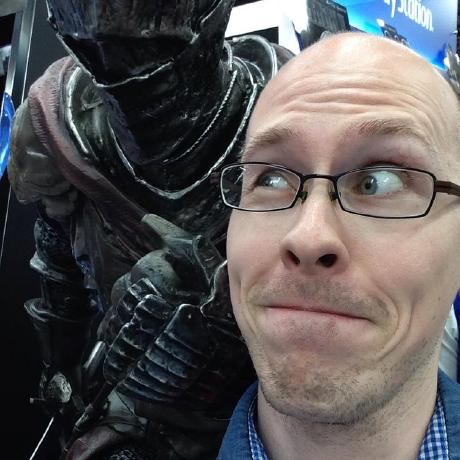
\includegraphics[width=\textwidth]{Lee.jpg}
\includegraphics[width=\textwidth]{Ben.png}
\column{0.15\textwidth}
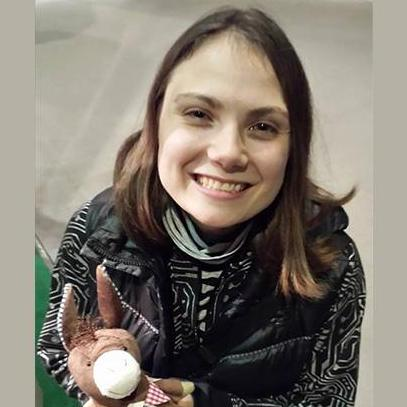
\includegraphics[width=\textwidth]{Irina.jpg}
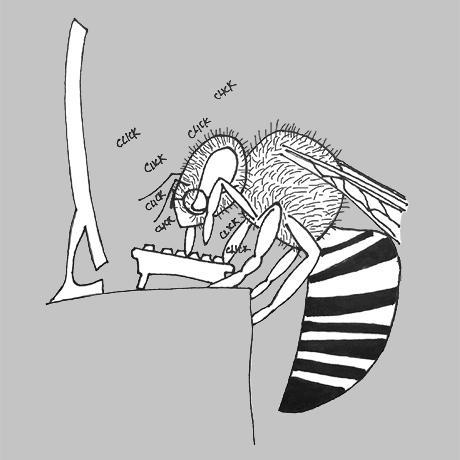
\includegraphics[width=\textwidth]{Valentin.jpg}
\column{0.15\textwidth}
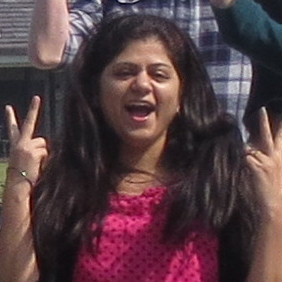
\includegraphics[width=\textwidth]{Rashi.jpg}
\includegraphics[width=\textwidth]{Peter.jpg}
\column{0.15\textwidth}
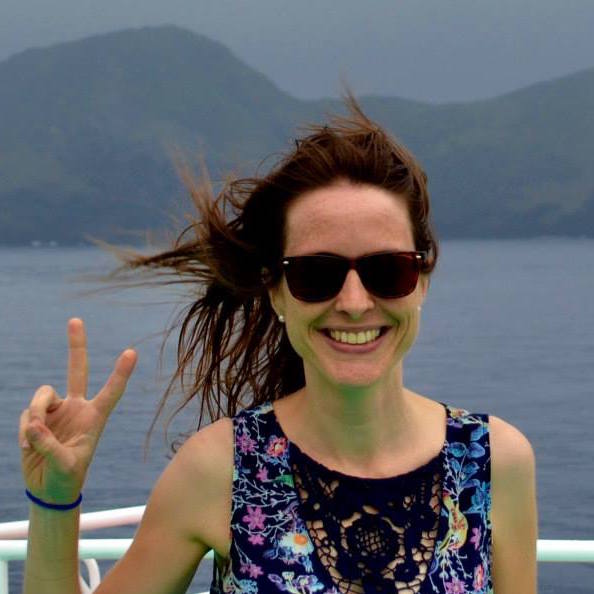
\includegraphics[width=\textwidth]{Angela.jpg}
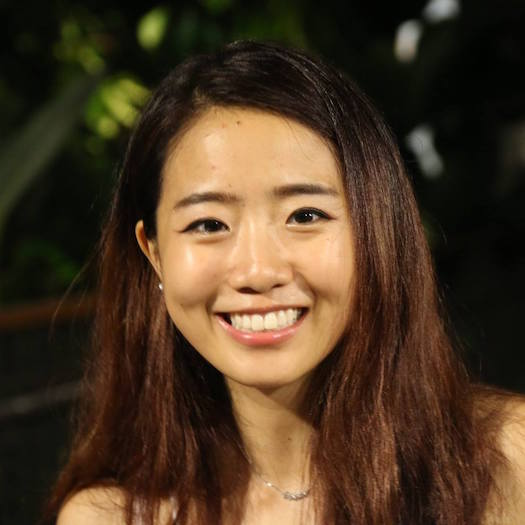
\includegraphics[width=\textwidth]{TT.jpg}
\column{0.15\textwidth}
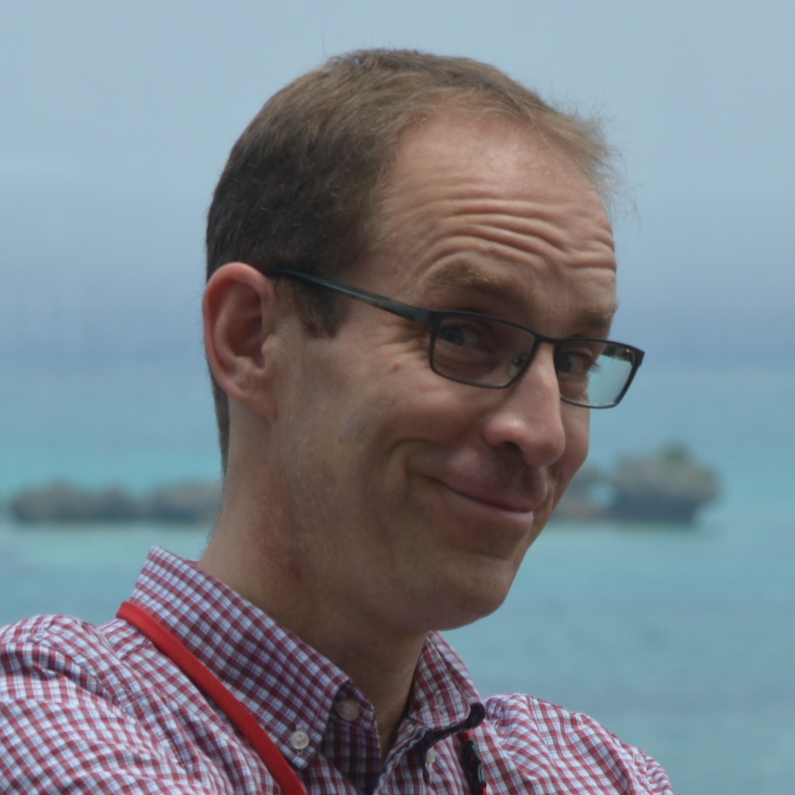
\includegraphics[width=\textwidth]{TB.JPG}
\column{0.03\textwidth}
\end{columns}
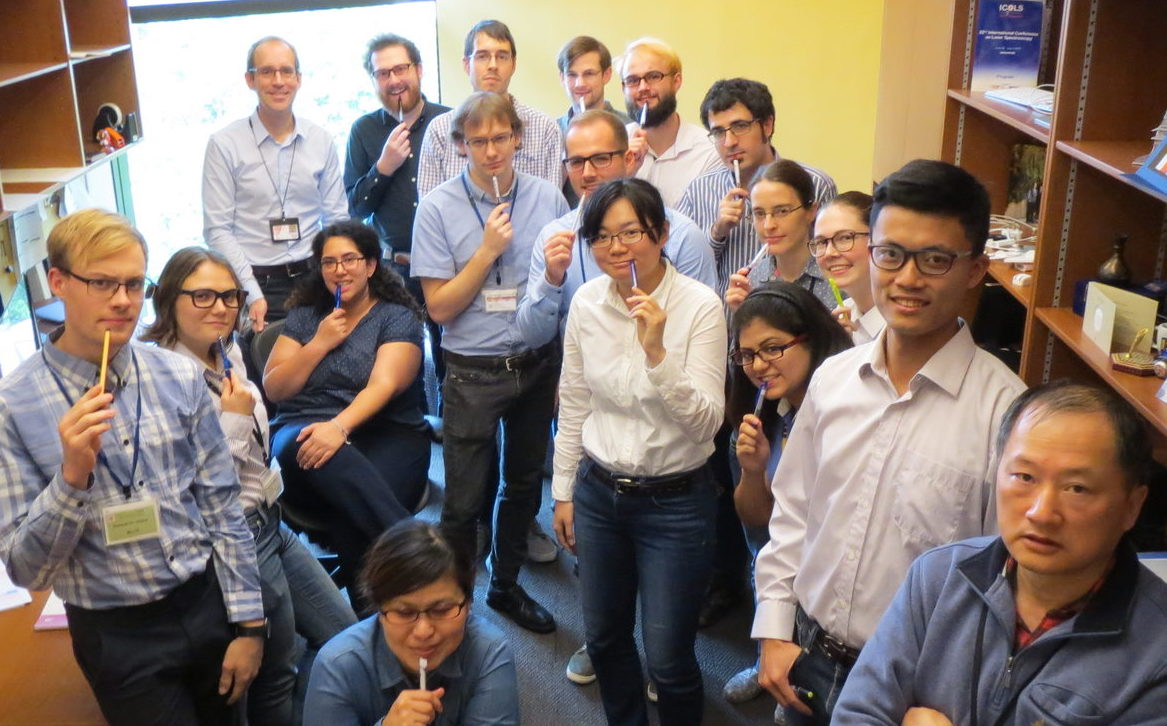
\includegraphics[width=\textwidth]{unit.JPG}
\column{0.3\textwidth}
Organizations:

\includegraphics[width=\textwidth]{OIST.png}

\includegraphics[width=\textwidth]{JSPS.png}
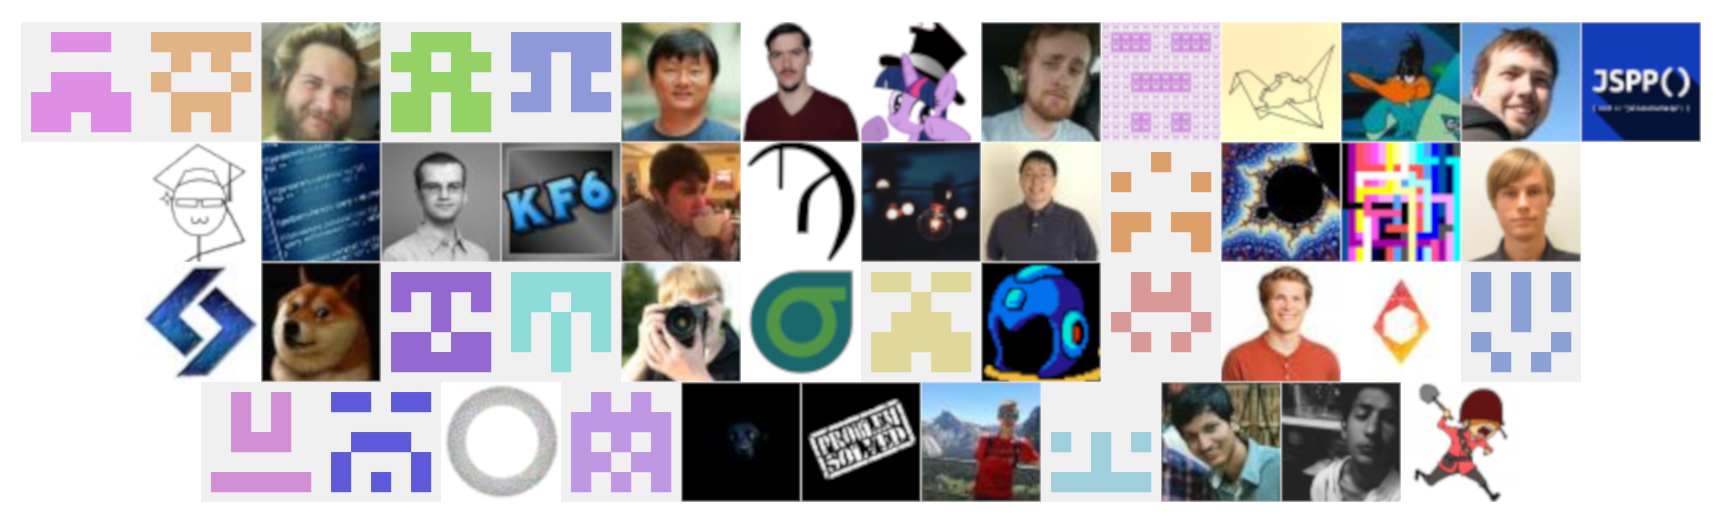
\includegraphics[width=\textwidth]{AAA.png}
\begin{center}
{\small algorithm-archive.org}
\end{center}
\end{columns}
\end{frame}

\begin{frame}
\frametitle{Conclusions}
\end{frame}

\begin{frame}
\center \huge Quantum state engineering
\end{frame}

\begin{frame}
\frametitle{Quantum optimal control}
Overall goal: optimize cost function by twiddling control parameters
\begin{columns}
\column{0.5\textwidth}
\begin{itemize}
\pause
\item Many known methods, such as \textbf{gradient descent}, \textbf{genetic algorithms}, and \textbf{machine learning}
\pause
\item For quantum systems, cost function is often the fidelity:
$$
\mathcal{F}= |\braket{\psi|\phi}|^2
$$
which required re-simulation every time a control parameter is changed
\end{itemize}
\pause
\column{0.5\textwidth}
\begin{center}
Nelder--Mead
\end{center}
\includegraphics[width=\textwidth]{../data/1d/NM/NM.pdf}

\end{columns}
\end{frame}

\begin{frame}
\frametitle{Example Tonks--Girardeau gas system}

\begin{columns}
\column{0.5\textwidth}
\begin{itemize}
\item NOON state: $\ket{N,0}+\ket{0,N}$

\item Tonks--Girardeau Gas: $g \rightarrow \infty$
\end{itemize}
\column{0.5\textwidth}
\begin{center}
\includegraphics[width = 0.7\textwidth]{../data/1d/scheme.pdf}
\end{center}
\end{columns}

\pause

\includegraphics[width = 0.49\textwidth]{../data/1d/cross.png}
\includegraphics[width = 0.49\textwidth]{../data/1d/nocross.png}
\end{frame}

\begin{frame}
\frametitle{CRAB method}

An example protocol is the Chopped RAndom Basis (CRAB) optimal control method where...

\begin{itemize}
\item A control parameter is modified with
$$
\Gamma^{\text{CRAB}}(t) = \Gamma^0(t)\gamma(t)
$$
where
$$
\gamma(t)=1+\frac{1}{\lambda(t)}\sum_{j=1}^J(A_j \sin(\nu_jt) + B_j\cos(\nu_jt))
$$
\item Works if $\lim_{t\rightarrow 0} \lambda(t) = \lim_{t\rightarrow T}\lambda(t) = \infty$
\item Creates a $3J$-dimensional space to optimize ($A, B, \nu$)
\end{itemize}

\end{frame}

\begin{frame}
\frametitle{STA protocol}
\includegraphics[width=\textwidth]{../data/1d/STAscheme.png}
\end{frame}

\begin{frame}
\frametitle{NOON optimization}

\begin{columns}
\column{0.5\textwidth}
\center Optimal control
\column{0.5\textwidth}
\center STA
\end{columns}

\begin{columns}
\column{0.5\textwidth}
\center \includegraphics[width=0.8\textwidth]{../data/1d/figlfid.pdf}
\column{0.5\textwidth}
\center \includegraphics[width=\textwidth]{../data/1d/fig6.png}
\end{columns}

\center Please ask questions at the end!
\end{frame}


\begin{frame}
\frametitle{Fidelities with optimal control}
\begin{columns}
\column{0.3\textwidth}
\begin{itemize}
\onslide<1->
\item Rotation ($\Omega(t)$)
\onslide<2->
\item Barrier height ($b(t)$)
\onslide<3->
\item Both
\end{itemize}
\column{0.7\textwidth}
\onslide<1->\includegraphics[width=.49\textwidth]{../data/1d/figR0.pdf}
\onslide<2->\includegraphics[width=.49\textwidth]{../data/1d/figB0.pdf}

\end{columns}

\begin{columns}
\column{0.3\textwidth}
\onslide<4->
\includegraphics[width=1.2\textwidth]{../data/1d/figlfid.pdf}
\column{0.7\textwidth}
\onslide<3->
\includegraphics[width=.49\textwidth]{../data/1d/figR1.pdf}
\includegraphics[width=.49\textwidth]{../data/1d/figB1.pdf}
\end{columns}
\end{frame}

\begin{frame}
\frametitle{NOON Optimization}
Optimizations of NOON state generation with 3 and 5 particles
\begin{center}
\includegraphics[width=0.49\textwidth]{../data/1d/figTG3.pdf}
\includegraphics[width=0.49\textwidth]{../data/1d/figTG5.pdf}
\end{center}
\end{frame}

\begin{frame}
\frametitle{STA protocol}
\includegraphics[width=\textwidth]{../data/1d/STAscheme.png}
\end{frame}

\begin{frame}
\frametitle{STA fidelities}
\begin{columns}
\column{0.5\textwidth}

\begin{itemize}
\onslide<1->
\item Fidelities with rotation
\onslide<2->
\item Fidelities with rotation of 100, 200 and higher particle number
\end{itemize}
\column{0.5\textwidth}
\onslide<1->
\includegraphics[width=\textwidth]{../data/1d/fig6.png}

\end{columns}

\onslide<2->
\begin{columns}
\column{0.5\textwidth}
\includegraphics[width=\textwidth]{../data/1d/fig7a.png}
\column{0.5\textwidth}

\includegraphics[width=\linewidth]{../data/1d/fig7b.png}
\end{columns}

\end{frame}


\begin{frame}
\frametitle{Cooley-Tukey}

\begin{columns}
\column{0.5\textwidth}
\begin{itemize}
\item Recursively subdivides DFT into simple sums with twiddle factors
\item Many known libraries, like FFTW, and CuFFT
\item Hard to parallelize (note for later)
\end{itemize}
\column{0.5\textwidth}
\includegraphics[width=\textwidth]{radix-8screen.jpg}
\end{columns}
\end{frame}


\begin{frame}
\frametitle{Distributed transpose}
\begin{columns}
\column{0.7\textwidth}
GPU transpose
\begin{itemize}
\item 2D out-of-place transpose $\approx$ copy \\
      \small{(shared memory, coalescence, bank conflicts)}
\item In-place transposes are inefficient
\item 3D permutations of arrays have 70\% efficiency
\onslide<2->
\item 2D distributed example
\end{itemize}

\column{0.3\textwidth}
\onslide<2->
\includegraphics[width=\textwidth]{transpose.png}
\center{\tiny Ruetsch, G. and Fatica, M. 2013}
\end{columns}
\end{frame}

\end{document}
